\documentclass[12pt]{extarticle}

%%%% paramètres généraux
%%%% french character
\usepackage[french]{babel}
\usepackage[T1]{fontenc}
\usepackage[utf8]{inputenc}

%%%% useful packages
\usepackage[a4paper, left=1.3cm, right=1.3cm, top=2.2cm, bottom=2.3cm]{geometry}
\usepackage{subcaption} % for figure caption
\usepackage{graphicx} % image
\usepackage{tabularx} % table
\usepackage{lastpage} %pour la définition de la dernière page
\usepackage[table]{xcolor} % color in table
\usepackage{amsmath} % math
\usepackage{amssymb} % bold math
\usepackage{wasysym} % integral
\usepackage[many]{tcolorbox} % colored box
\usepackage{awesomebox} % pour des box déjà définies
\usepackage{fancyhdr} % headers
\usepackage{enumitem} % for bullet in itemize
\usepackage[colorlinks=true,linkcolor=black,citecolor=black,filecolor=black,urlcolor=black]{hyperref} % for link
\usepackage[backend=biber,style=alphabetic,sorting=ynt]{biblatex}
\usepackage{accents} % for complex notation
\usepackage[european, straightvoltages, RPvoltages]{circuitikz} % for electronic circuit

\usepackage{hyperref}   %pour les liens url et les références
\hypersetup{
    colorlinks=true,
    urlcolor=blue,
    linkcolor=blue,
    breaklinks=true
}
\usepackage{empheq}
\usepackage{multicol} % to use several columns
%\setlength{\columnseprule}{1pt} %Separator ruler width
\usepackage{cellspace}  % espace du texte dans les colonnes tableaux
\usepackage{colortbl}  %pour colorier les cases de tableaux
\tcbuselibrary{skins} %library de 
\usepackage{shadow}
\usepackage{pifont}

\usepackage{fontawesome5}

%\usepackage{fontawesome} % awesome icons
\usepackage{ifthen} % for loop and boolean in commands
\usepackage{qrcode}
\usepackage{pdfpages} % to include pdf
\usepackage{wrapfig} % to wrap text around figures
\usepackage{chemfig} % to draw chemistry formula
\usepackage{chemist} % surtout pour chemform
\usepackage{multirow} % for vertically merged cells
\usepackage{makecell} % to format cell in tables
\usepackage{physics} % for derivatives, braket, etc.
\usepackage{esvect} % for large vectors
\usepackage{listings} % for code
\usepackage{dashundergaps} % for automatic text to fill
% dyslexia friendly font (need to be compiled in xetex)
%\usepackage{fontspec}
%\setmainfont{OpenDyslexic}
\usepackage{tikz}
\usepackage{pgfplots}
\usepackage[framemethod=tikz]{mdframed} %pour les boîtes
\usepackage{dashundergaps} %pour les textes à trous

%%%% settings
\setlength{\parskip}{0cm}
\setlength{\parindent}{0cm}
\renewcommand{\baselinestretch}{1.3}
\setcounter{tocdepth}{2}
\renewcommand{\thesection}{\textcolor{red}{\Roman{section}}}
\renewcommand{\thesubsection}{\textcolor{red}{\Roman{section}.\arabic{subsection}}}

%%%% tikz configuration
\usetikzlibrary{babel}
\tikzset{>=latex}
\usetikzlibrary{shadows}
\usetikzlibrary{backgrounds}



%%%% header
\renewcommand{\headrulewidth}{0.4pt}
\setlength{\headheight}{22.50113pt}


%%%% Table
\renewcommand{\tabularxcolumn}[1]{m{#1}}
\setlength{\extrarowheight}{8pt}
\newcolumntype{P}[1]{>{\centering\arraybackslash}p{#1\linewidth}}% colonne de type p mais centrée
\cellspacetoplimit 2pt %espace au dessus du texte
\cellspacebottomlimit 2pt  %espace en dessous du texte



%%%% Chemfig configuration
\setchemfig{
  atom sep=20pt,
  bond style={line width=1pt},
  angle increment=30
}


%%%% dashundergaps configuration
\dashundergapssetup{
  gap-numbers = false,
  gap-format = dot,
  gap-widen,
  gap-extend-percent
}


%\bibliographystyle{plain}
\bibliography{TSNR/TSNR.bib}

%%%% quelques commandes
%%%%%%%%%%%%%%%%%%%%%%%%%%%%%%%%%%%%%%%%%%%%%%%%%%%%%%%%%%%%%%%%%%%%%%%%%%
%%%% quelque couleurs
\definecolor{vertSombre} {RGB}{  0,  92,  46}
\definecolor{cyanSombre} {RGB}{  0, 140, 128}
\definecolor{jauneSombre}{RGB}{138, 103,   0}
\definecolor{jauneClair} {RGB}{218, 173,   0}
\definecolor{rougeSombre}{RGB}{148,  31,   0}
\definecolor{rougeClair} {RGB}{224,  39,  34}
\definecolor{couleurtitre}{RGB}{255,  255,  255}
\definecolor{exef}{RGB}{210,210,210}
\definecolor{propositiono}{RGB}{109,109,109}

%%% quelques couleurs dérivées des couleurs choisie
\newcommand{\couleurCorrection}{couleurPrincipale!60!black}
\newcommand{\couleurExercice}{couleurPrincipale!75!black}

%%%% rectangle coloré
\newcommand\rectangle[3]{%
  \shorthandoff{;}
  \tikz \node (rect) [draw, fill, color=#1,
              minimum width=#2,
              minimum height=#3] {};
  \shorthandon{;}
}
\newcommand\rectangleCyan[2]{\rectangle{couleurPrincipale}{#1}{#2}}

%%%% simple boite
\newenvironment{boite}{
  \begin{tcolorbox}
  [ breakable, enhanced jigsaw, % to break box over page
    arc = 0mm, % straight line
    colback= white, % white background
    colframe= black % dark frame
  ]
}
{ \end{tcolorbox} }

\newtcolorbox{facile}[2][]{colback=green!5!white,
colframe=green!75!black,fonttitle=\bfseries,
colbacktitle=green!85!black,enhanced,
attach boxed title to top center={yshift=-2mm},
title={#2},#1}

\newtcolorbox{difficile}[2][]{colback=red!5!white,
colframe=red!75!black,fonttitle=\bfseries,
colbacktitle=red!85!black,enhanced,
attach boxed title to top center={yshift=-2mm},
title={#2},#1}


%\newenvironment[1]{Propriete}{\begin{tcolorbox}[colback=red!5!white,colframe=red!75!black,title=\textbf{#1 :}]
%}
%{\end{tcolorbox} 


%%%%%%%%%%%%%%%%%%%%%%%%%%%%%%%%%%%%%%%%%%%%%%%%%%%%%%%%%%%%%%%%%%%%%%%%%%
%%%% pagination et sections
\newcommand{\titre}[1]{
  \begin{center}
    \textsf{\bfseries \Large #1}
  \end{center}
}
\newcommand{\sousTitre}[1]{
  \textsf{\bfseries #1}
}
\newcommand{\pasDePagination}{
  \thispagestyle{empty}
}
\newcommand{\feuilleBlanche}{
  \newpage
  \phantom{b}
  \pasDePagination
}


%%%% activité ou TP
\newcounter{acti}
\newcommand{\titreActi}[2]{
  \refstepcounter{acti}
  \titre{#1 \arabic{section}.\arabic{acti} -- #2}
}
\newcommand{\titreTP}[1]{
  \titreActi{TP}{#1}
  %\titreActi{Activité expérimentale}{#1}
}
\newcommand{\titreActivite}[1]{
  \titreActi{Activité}{#1}
}
\newcommand{\titreEvaluation}[1]{
  \titreActi{Évaluation}{#1}
}


%%%% chapitre, section et sous-section
\newcommand{\titreChapitre}[1]{
  \titre{Chapitre \arabic{section} : #1}
}
\newcommand{\titrePartie}[1]{
  \vspace*{24pt}
  \refstepcounter{subsection}
  \rectangleCyan{60pt}{1pt}
  \sousTitre{\Large \Roman{subsection} -- #1}
  \rectangleCyan{60pt}{1pt}
  \vspace*{10pt}
}
\newcounter{sousSection}
\newcommand{\titreSection}[1]{
  \vspace*{16pt}
  \refstepcounter{subsubsection}
  \setcounter{sousSection}{0}
  \rectangleCyan{30pt}{4pt}
  \sousTitre{\large \arabic{subsubsection} -- #1}
  \vspace*{10pt}
}
\newcommand{\titreSousSection}[1]{
  \vspace*{12pt}
  \refstepcounter{sousSection}
  \sousTitre{\Alph{sousSection} -- #1}
  \vspace*{8pt}
}

%%%% fixe le numéro de l'activité
\newcommand{\numeroActivite}[1]{
  \setcounter{subsection}{0}
  \setcounter{subsubsection}{0}
  \setcounter{sousSection}{0}
  \setcounter{figure}{0}
  \setcounter{document}{0}
  \setcounter{exercice}{0}
  \setcounter{QCM}{0}
  \setcounter{countCoupDePouce}{0}
  \setcounter{acti}{#1 - 1}
  \setcounter{page}{1}
}
% fixe le numéro de page (#2) et de partie (#1)
\newcommand{\numeroPartieCours}[2]{
  \newpage
  \setcounter{subsection}{#1 - 1}
  \setcounter{page}{#2}
}

%%%% lignes
\newcommand{\ligne}{
  \par\noindent\rule{\textwidth}{0.4pt}
}
\newcommand{\lignePointillee}[1]{
  \makebox[#1\textwidth]{\dotfill}
}


%%%%%%%%%%%%%%%%%%%%%%%%%%%%%%%%%%%%%%%%%%%%%%%%%%%%%%%%%%%%%%%%%%%%%%%%%%
%%%% en-tête
\newcommand{\teteGauche}[1]{
  \lhead{
    \textbf{\footnotesize #1}
  }
}
\newcommand{\teteDroite}[1]{
  \rhead{
    \hfill \textbf{\footnotesize #1}
  }
}

%

\newcommand{\enTeteRevision}[2]{
  \pagestyle{fancy}
  \lhead{Revision #1 - \textit{#2}}
  %\chead{} % central header
  \teteDroite{Lycée Parc de Vilgénis 2023 - 2024}
}

\newcommand{\enTeteMethodo}[2]{
  \pagestyle{fancy}
  \teteGauche{Fiche Méthode #1 : #2}
  %\chead{} % central header
  \teteDroite{Lycée Parc de Vilgénis 2023 - 2024}
}

\newcommand{\enTeteChap}[2]{
  \pagestyle{fancy}
  \lhead{Chapitre #1 - \textit{#2}}
  %\chead{} % central header
  \teteDroite{Lycée Parc de Vilgénis 2023 - 2024}
}

\newcommand{\enTeteExo}[1]{
  \pagestyle{fancy}
  \lhead{Exercices du Chapitre #1}
  %\chead{} % central header
  \teteDroite{Lycée Parc de Vilgénis 2023 - 2024}
}

\newcommand{\enTeteAct}[3]{
  \pagestyle{fancy}
  \lhead{Chapitre #1 \newline Activité #2 - \textit{#3}}
  %\chead{} % central header
  \teteDroite{Lycée Parc de Vilgénis 2023 - 2024}
}

\newcommand{\enTeteDM}[2]{
  \pagestyle{fancy}
  \lhead{Devoir Maison n$\degree$ #1 - \textit{#2}}
  %\chead{} % central header
  \teteDroite{Lycée Parc de Vilgénis 2023 - 2024}
}

\newcommand{\enTeteTP}[2]{
  \pagestyle{fancy}
  \lhead{TP #1 - \textit{#2}}
  %\chead{} % central header
  \teteDroite{Lycée Parc de Vilgénis 2023 - 2024}
}
%
\newcommand{\enTeteSeance}[2]{
  \pagestyle{fancy}
  \lhead{Date : \textit{#1}}
  \chead{Séance : #2}
  \teteDroite{Seconde} % central header
}
%

\newcommand{\enTeteFicheReussite}[1]{
  \newpage
  \setcounter{subsection}{0}
  \pasDePagination
  
  \phantom{b}
  \vspace*{-70pt}
  \titre{Fiche \og Réussir son évaluation \fg}
  \titre{#1}
  
  \vspace*{-6pt}
  % \titreSection{Ce que je dois savoir}
  
  Pour savoir quoi réviser, je lis les points clés du chapitre évalués :
  \begin{itemize}
    \item Si je pense maîtriser une notion, je coche la case \ok
    \item Si je pense que je dois la retravailler, je coche la case \pasOk
  \end{itemize}
  
  Pour travailler les notions qui ne sont pas maîtrisées, je reprend les activités associés.
}
\newcommand{\basDePageFicheReussite}{
  \titreSection{Ce qu'il me reste à faire}
}
\newcommand{\travailExerciceCorrige}{
  Pour être sûr-e d'obtenir une bonne note, je m'entraîne avec les exercices corrigés du manuel indiqués dans la colonne de droite.
}
\newcommand{\questionFicheReussite}[1]{
  S'il me reste des questions, je les note ici pour les poser au début de l'évaluation :\\[4pt]
  \lignesReponse{#1}
}
\newcommand{\coursFicheReussite}{
  Je prépare une fiche au format A4 avec toutes les notions, définitions ou grandeurs dont je pense avoir besoin pendant l'évaluation.
}


%%%%%%%%%%%%%%%%%%%%%%%%%%%%%%%%%%%%%%%%%%%%%%%%%%%%%%%%%%%%%%%%%%%%%%%%%%
%%%% exercice
% définit un booléen pour entrer ou sortir du mode correction
\newboolean{modeProf}
\setboolean{modeProf}{false}
\newcommand{\modeCorrection}{
  \setboolean{modeProf}{true}
  \TeacherModeOn
}

% définit une commande pour afficher une question 
% #1 : question
% #2 : réponse
% #3 : nombres de lignes pour répondre
\newcommand{\question}[3]{
  \numeroQuestion\!#1
  
  % pointille ou correction
  \ifthenelse {\boolean{modeProf}} { % prof
    \reponseCorrigee{#2}
  }{ % eleve
    \vspace*{8pt}
    \lignesReponse{#3}
  }
}

%
\newcounter{exercice}
\newcommand{\numeroQuestion}{
  \refstepcounter{exercice}
  \vspace*{2pt}
  \hspace{15pt}
  \textcolor{black}{%couleurPrincipale!75!black}{
    \textbf{\arabic{exercice}} {\small\faMinus}
  }
}

% correction
\newcommand{\reponseCorrigee}[1]{
  \vspace*{2pt}
  \hspace{16pt}
  \textcolor{red}{
    \faCaretRight \hspace{2pt} #1
  }
}
\newcommand{\correction}[1]{
  \ifthenelse {\boolean{modeProf}} { % prof
    \textcolor{red}{#1}
  }{ % eleve
  }
}

% trace des lignes pour répondre
\newcounter{int}
\newcommand{\lignesReponse}[1]{
  \setcounter{int}{-1}
  \loop
    \stepcounter{int}
    \ifnum \value{int} < #1
    \lignePointillee{0.99} \\[8pt]
  \repeat
  \ifnum #1 > 0
    \vspace*{-12pt}
  \fi
}

% sous questions
\newcommand{\sousQuestion}[2]{
  \hspace{15pt}
  \textcolor{couleurPrincipale!75!black}{\textbullet} #1
  
  \vspace*{8pt}
  \reponse{#2}
}


%%%%%%%%%%%%%%%%%%%%%%%%%%%%%%%%%%%%%%%%%%%%%%%%%%%%%%%%%%%%%%%%%%%%%%%%%%
%%%% QCM
% question QCM
\newcounter{QCM}
\newcommand{\QCM}[2]{
  \refstepcounter{QCM}
  \vspace*{2pt}
  \textcolor{couleurPrincipale!75!black}{\textbf{\arabic{QCM}} {\small\faMinus}} #1
  
  \begin{qcm}
    #2
  \end{qcm}
}


%%%% Pour afficher les compétences
\newcommand{\competence}[1]{
  ~{\footnotesize\textit{(#1)}}
}


%%%% Espace pour indiquer nom, prénom et classe
\newcommand{\nomPrenomClasse}{
  \vspace*{-24pt}
  \underline{Nom} : \lignePointillee{0.3}\hfill \underline{Date } : \gap{....}/\gap{....}/\gap{....} \newline 
  \underline{Prénom} : \lignePointillee{0.3} \hfill\underline{Classe} : \gap{........}
}


%%%%%%%%%%%%%%%%%%%%%%%%%%%%%%%%%%%%%%%%%%%%%%%%%%%%%%%%%%%%%%%%%%%%%%%%%%
% texte à trou automatique
\newcommand{\texteTrouAuto}[1]{
  \gap{
    \textcolor{couleurPrincipale!60!black}{ \textbf{#1} }
  }
}

% texte à trou dans une ligne réglable
\newcommand{\texteTrou}[2]{
  \ifthenelse {\boolean{modeProf}} {% prof
    \textcolor{couleurPrincipale!60!black}{ \textbf{#1} }
  }{% élève
    \espaceReponse
    \lignePointillee{#2}
  }
}

% texte à trou sur plusieurs lignes
\newcommand{\texteTrouLigneComplete}[1]{
  \ifthenelse {\boolean{modeProf}} {% prof
    \textcolor{couleurPrincipale!60!black}{ \textbf{#1} }
  }{% élève
    \espaceReponse \dotfill
  }
}

% texte à trou sur plusieurs lignes
\newcommand{\texteTrouMultiLignes}[2]{
  \ifthenelse {\boolean{modeProf}} {% prof
    \textcolor{couleurPrincipale!60!black}{ \textbf{#1} }
  }{% élève
    \reponseLigne
    \lignesReponse{#2}
  }
}

% reponse en fin de ligne
\newcommand{\reponseLigne}{
  \espaceReponse
  \dotfill \\[8pt]
}

% espace vertical pour la réponse
\newcommand{\espaceReponse}{
  \phantom{$\Frac{1}{1}$} % espace vertical
  \hspace*{-40pt} \phantom{b} % ajuste l'espace horizontal
}

%%%%%%%%%%%%%%%%%%%%%%%%%%%%%%%%%%%%%%%%%%%%%%%%%%%%%%%%%%%%%%%%%%%%%%%%%%
%%%% Pour choisir parmi deux sujets
\newboolean{sujetA}
\setboolean{sujetA}{true}
\newcommand{\sujetB}{
  \setboolean{sujetA}{false}
}
\newcommand{\sujetA}{
  \setboolean{sujetA}{true}
}

%%%% Pour faire plusieurs sujets en parallèle
\newcommand{\variationSujet}[2]{
  \ifthenelse {\boolean{sujetA}}
  {\hspace*{-2pt}#1\hspace*{-2pt}}
  {\hspace*{-2pt}#2\hspace*{-2pt}}
}


%%%%%%%%%%%%%%%%%%%%%%%%%%%%%%%%%%%%%%%%%%%%%%%%%%%%%%%%%%%%%%%%%%%%%%%%%%
%%%% documents
\newcounter{document}
\newcommand{\titreDocu}[1]{
  \refstepcounter{document} % update counter
  \textbf{Document \arabic{document} -- #1} % print document title
  \addcontentsline{toc}{document}{\protect\numberline{} #1} % update table of content
}
\newenvironment{doc}[1]{
  \begin{boite}
    \titreDocu {#1} \newline
}
{ \end{boite} }

%\newenvironment{exo}[1]{
%\begin{mdframed}[style=autreexo]
%\textbf{\bsc{Exercice de cours 1} - Espèces chimiques}\\
%Donner le type (\textit{atomique}, \textit{moléculaire} ou \textit{ionique}) des espèces chimiques suivantes : hélium (He), eau (H\textsubscript{2}O), chlorure de sodium (Na$^{+}$, Cl$^{-}$).
%\end{mdframed}
%}
%% pour les référencer
\newcommand{\docu}[1]{
  \textbf{(Doc. #1)}
}


%%%% problematique
\newcommand{\problematique}[1]{
  %\hspace{8pt}
  \noindent\textcolor{red}{\begin{large} \textbf{\underline{Problématique} : }\end{large}}\textbf{#1}
  }



%%%% objectifs
\newenvironment{objBoite}{
  \begin{tcolorbox}
  [boxrule = 0pt,
  frame hidden, sharp corners,
  colback = white, enhanced,
  borderline north={2pt}{0pt}{couleurPrincipale},
  borderline south={2pt}{0pt}{couleurPrincipale},
  borderline west={4pt}{0pt}{couleurPrincipale},
  borderline east={4pt}{0pt}{couleurPrincipale}
  ]
  
}
{
  \end{tcolorbox}
}
\newenvironment{objectifs}{
  \begin{objBoite}
    \begin{center}
      \sousTitre{\large Objectifs de la séance :}
      \begin{listeObjectifs}
}
{ 
      \end{listeObjectifs}
    \end{center}
  \end{objBoite}
}

%%%% Espace pour un coup de pouce
\newcounter{countCoupDePouce}
\newenvironment{coupDePouce}{
  \refstepcounter{countCoupDePouce}
  \vspace*{-12pt}
  \begin{boite}
    \begin{flushright}
      \textcolor{couleurPrincipale}{\faSquareO}
    \end{flushright}
    
    \vspace*{-30pt}
    \textcolor{couleurPrincipale}{\faThumbsUp}
    \textbf{Coup de pouce \arabic{countCoupDePouce}} :\\[4pt]
}
{
  \end{boite}
}


%%%% Espace pour une appréciation
\newcommand{\appreciation}[1]{
  \vspace*{8pt}
  \sousTitre{Appréciation et remarques}
  \vspace*{-8pt}
  \begin{boite}
    \vspace{#1 pt}
    \phantom{b}
  \end{boite}
}


%%%%%%%%%%%%%%%%%%%%%%%%%%%%%%%%%%%%%%%%%%%%%%%%%%%%%%%%%%%%%%%%%%%%%%%%%%
%%%% Définit un nouveau type de colonne : taille fixée par une fraction
%%%% de la largeur de la ligne, avec un texte centré
\newcolumntype{C}[1]{>{\centering\arraybackslash}p{#1\linewidth}}

%%%% Tableau de competence
\newenvironment{tableauCompetences}{
  \centering
  \setlength{\extrarowheight}{6pt}
  \tabularx{\linewidth}{| c | X | c | c | c | c |}
    \hline
    \rowcolor{blue!25}
    \centering \textbf{Compétences} & \centering \textbf{Items} & \textbf{D} & \textbf{C} & \textbf{B} & \textbf{A}
    \\ \hline
}
{
    \\ \hline
  \endtabularx
}

%%%% Tableau de connaissances
\newenvironment{tableauConnaissances}{
  \centering
  \setlength{\extrarowheight}{6pt}
  \tabularx{\linewidth}{| X | c | c | C{0.18} | C{0.15} |}
    \hline
    \rowcolor{gray!20} 
    \textbf{Points clés du chapitre} & \ok & \pasOk & \textbf{En classe} & \textbf{Exercices}
    \\ \hline
}
{   
    \\ \hline
  \endtabularx
}

%%%% Tableau de connaissances sans exercices
\newenvironment{tableauConnaissancesSansExercices}{
  \centering
  \setlength{\extrarowheight}{6pt}
  \tabularx{\linewidth}{| X | c | c | C{0.2} |}
    \hline
    \rowcolor{gray!20} 
    \textbf{Points clés du chapitre} & \ok & \pasOk & \textbf{En classe}
    \\ \hline
}
{   
    \\ \hline
  \endtabularx
}

%%%% Tableau de correction élève
\newcommand{\correctionEleve}[1]{
  \setlength{\extrarowheight}{6pt}
  \begin{tabularx}{\linewidth}{| X | C{0.26} | C{0.26} | C{0.26} |}
    \hline
    \rowcolor{gray!20}
    \textbf{Question} &
    \textbf{L'erreur} &
    \textbf{Analyse de l'erreur} &
    \textbf{La correction}
    \\ \hline
    %
    \phantom{b} \vspace{#1 pt}
    & & & \\ \hline
    \phantom{b} \vspace{#1 pt}
    & & & \\ \hline
    \phantom{b} \vspace{#1 pt}
    & & & \\ \hline
    \phantom{b} \vspace{#1 pt}
    & & & \\ \hline
  \end{tabularx}
}

%%%% Tableau bilan de la correction
\newcommand{\bilanCorrection}[1]{
  \setlength{\extrarowheight}{6pt}
  \begin{tabularx}{\linewidth}{| X | X |}
    \hline
    \rowcolor{gray!20}
    \textbf{Ce que je n'avais pas compris...} &
    \textbf{Ce que maintenant j'ai compris...}
    \\ \hline
    \phantom{b} \vspace{#1 pt} % \newline \newline \newline
    & \\ \hline
  \end{tabularx}
}


%%%%%%%%%%%%%%%%%%%%%%%%%%%%%%%%%%%%%%%%%%%%%%%%%%%%%%%%%%%%%%%%%%%%%%%%%%
%%%% symboles : chevron, flèche, attention, etc.
\newcommand{\chevron}{
  \textcolor{couleurPrincipale}{\small \faChevronRight}
}
%
\newcommand{\fleche}{
  \textcolor{couleurPrincipale}{\faCaretRight}
}
%
\newcommand{\attention}{
  \textcolor{couleurPrincipale}{\faExclamationTriangle}
}
%
\newcommand{\flecheLongue}{
  \textcolor{red}{\longrightarrow}
}
%
\newcommand{\ok}{
  \textcolor{couleurPrincipale}{\faCheckCircle}
}
%
\newcommand{\pasOk}{
  \textcolor{couleurPrincipale}{\faTimesCircle}
}
%
\newcommand{\pointCyan}{
  \textcolor{couleurPrincipale}{\textbullet}
}
%
\newcommand{\mesure}{
  \hspace{15pt}
  \textcolor{couleurPrincipale!75!black}{\faWrench\faFlask}
}


%%%%%%%%%%%%%%%%%%%%%%%%%%%%%%%%%%%%%%%%%%%%%%%%%%%%%%%%%%%%%%%%%%%%%%%%%%
%%%% Passage important
\newenvironment{definition}[1]{
  \begin{tcolorbox}[colback=green!5!white,colframe=green!75!black,title=\textbf{#1}]
  
}
{
  \end{tcolorbox}
}

%%%% contexte
\newenvironment{contexte}{
  \begin{tcolorbox}
  [boxrule = 4pt, sharp corners,
  colframe = couleurPrincipale,
  colback = white!95!couleurPrincipale, % background color
  breakable, enhanced jigsaw] % to break box over page
  
}
{
  \end{tcolorbox}
}


%%%% emphase
\newcommand{\emphase}[1]{
  \textcolor{couleurImportant}{\textsf{\bfseries \large #1}}
}
%
\newcommand{\important}[1]{
  \!\textcolor{green}{\textbf{\bfseries #1}}\!\!
}
%
\newcommand{\exemple}{
  \flecheLongue \textit{Exemple :}
}
\newcommand{\exemples}{
  \flecheLongue \textit{Exemples :}
}
%
\newcommand{\note}{
  \textbf{Note :}
}
%
\newcounter{appelProf}
\newcommand{\appelProf}{
  \refstepcounter{appelProf}
  \hspace{24pt} \faHandPaperO \hspace{2pt}
  \textbf{Appel n$^\circ$ \arabic{appelProf} :}
}


%%%% image
\newcommand{\image}[2]{
  \includegraphics[width=#1\linewidth]{#2}
}


%%%%%%%%%%%%%%%%%%%%%%%%%%%%%%%%%%%%%%%%%%%%%%%%%%%%%%%%%%%%%%%%%%%%%%%%%%
%%%% qcm
\newlist{qcm}{itemize}{2}
\setlist[qcm]{label=$\square$, leftmargin=2cm}


%%%% liste d'objectif
\newlist{listeObjectifs}{itemize}{2}
\setlist[listeObjectifs]{label = \chevron}


%%%% protocole
\newlist{protocole}{itemize}{2}
\setlist[protocole]{label = {\footnotesize \fleche}}


%%%% liste de points
\newlist{listePoints}{itemize}{2}
\setlist[listePoints]{label = \pointCyan}


%%%% jeu de données
\newenvironment{donnees}{
  \textbf{Données :}
  \begin{listePoints}
}{
  \end{listePoints}
}


%%%% liste avec chiffre
\newlist{enumeration}{enumerate}{2}
\setlist[enumeration]{label = \textcolor{couleurPrincipale!75!black}{\textbf{\arabic*.}} }


%%%%%%%%%%%%%%%%%%%%%%%%%%%%%%%%%%%%%%%%%%%%%%%%%%%%%%%%%%%%%%%%%%%%%%%%%%
%%%% Séparation de la page
\newcommand{\separationTroisBlocs}[3]{
  \begin{minipage}[t]{0.3\linewidth}
    #1
  \end{minipage}
  ~
  \begin{minipage}[t]{0.3\linewidth}
    #2
  \end{minipage}
  ~
  \begin{minipage}[t]{0.3\linewidth}
    #3
  \end{minipage}
}
%%%%
\newcommand{\separationDeuxBlocs}[2]{
  \begin{minipage}[t]{0.48\linewidth}
    #1
  \end{minipage}
  \hfill
  \begin{minipage}[t]{0.48\linewidth}
    #2
  \end{minipage}
}
\newcommand{\separationBlocs}[4]{
  \begin{minipage}[t]{#1\linewidth}
    #3
  \end{minipage}
  \hfill
  \begin{minipage}[t]{#2\linewidth}
    #4
  \end{minipage}
}


%%%%%%%%%%%%%%%%%%%%%%%%%%%%%%%%%%%%%%%%%%%%%%%%%%%%%%%%%%%%%
%%%% tikz macros
%%%% rectangle
\newcommand{\tkzRect}[4]{
  \fill[color=#1] (#2,#4) -- (-#2,#4) -- (-#2,#3) -- (#2,#3);
}
\newcommand{\tkzEllipse}[4]{
  \fill[color=#1] (0,#3) ellipse (#2 and #4);
}
\newcommand{\tkzLegende}[4]{
  \draw[black, ->, very thick] (#2 + #4, #3) node[right] {#1} -- (#2, #3);
}
\newcommand{\tkzCercle}[4]{
  \filldraw [#3] (#1, #2) circle (#4pt);
}
\newcommand{\tkzCercleLigne}[5]{
  \filldraw [color = #4, fill = #3, very thick] (#1, #2) circle (#5pt);
}
%%%% tube à essais
\newcommand{\tkzTubeEssai}[3]{
  \draw[thick] (#1,#2) -- (#1,0) arc (0:-180:#1) -- (-#1,#2);
  \draw[thick] (0,#2) ellipse (#1 and #3);
}
\newcommand{\tkzBasTubeEssai}[5]{
  \fill[color=#1] (-#2,#3) -- (#2,#3) arc (0:-180:#2);
  \tkzRect{#1}{#2}{#3 - 0.01}{#4}
  \tkzEllipse{#1!85!black}{#2}{#4}{#5}
}
\newcommand{\tkzPhaseTubeEssai}[5]{
  \tkzRect{#1}{#2}{#3}{#4}
  \tkzEllipse{#1}{#2}{#3}{#5}
  \tkzEllipse{#1!85!black}{#2}{#4}{#5}
}

%%%% Point et vecteurs
\newcommand{\tkzLabel}[3]{
  \node at (#1, #2) {#3};
}
\newcommand{\tkzPointLabel}[3]{
  \filldraw (#1, #2) circle (2pt) node[above] {#3};
}
\newcommand{\tkzVecteur}[6]{
  \draw[black, ->, very thick] (#1, #2) -- (#1 + #3, #2 + #4) node[#6] {#5};
}
\newcommand{\tkzEquiv}[6]{
  \draw[black, <->, thick] (#1, #2) -- (#1 + #3, #2 + #4);
  \draw[black] (#1 + #3/2, #2 + #4/2) node[#6] {#5};
}
\newcommand{\tkzVecteurX}[4]{
  \draw[black, ->, very thick] (#1, #2) -- (#1 + #3, #2) node[above] {#4};
}
\newcommand{\tkzVecteurY}[4]{
  \draw[black, ->, very thick] (#1, #2) -- (#1, #2 + #3) node[right] {#4};
}
\newcommand{\tkzEquivY}[5]{
  \draw[#1, <->, thick] (#2, #3) -- (#2, #3 + #4);
  \draw[#1] (#2, #3 + #4/2) node[right] {#5};
}
\newcommand{\tkzEquivX}[5]{
  \draw[#1, <->, thick] (#2, #3) -- (#2 + #4, #3);
  \draw[#1] (#2 + #4/2, #3) node[below] {#5};
}

%%%% plan de classe
\newcommand{\rectangleTexte}[5]{
  \filldraw [fill=white, draw=black, ultra thick] (#1, #2) rectangle (#1 + #3, #2 + #4);
  \node at (#1 + #3/2, #2 + #4/2) [font=\sffamily] {\textbf{\large #5}};
}
% place dans la classe
\newcommand{\place}[3]{
  \rectangleTexte{#1}{#2}{3}{2}{#3}
}
\newcommand{\deuxPlaces}[4]{
  \place{#1}{#2}{#3}
  \place{#1 + 3}{#2}{#4}
}
\newcommand{\troisPlaces}[5]{
  \place{#1}{#2}{#3}
  \place{#1 + 3}{#2}{#4}
  \place{#1 + 6}{#2}{#5}
}
\newcommand{\quatrePlaces}[6]{
  \place{#1}{#2}{#3}
  \place{#1 + 3}{#2}{#4}
  \place{#1 + 6}{#2}{#5}
  \place{#1 + 9}{#2}{#6}
}
%%%% rangée
\newboolean{quatrePlace}
\setboolean{quatrePlace}{false}
\newcommand{\avecQuatrePlaces}{ \setboolean{quatrePlace}{true} }
\newcommand{\avecTroisPlaces}{ \setboolean{quatrePlace}{false} }
\newcommand{\rangee}[9]{
  \ifthenelse {\boolean{quatrePlace}} {
    \deuxPlaces  {0}{#1} {#2}{#3}
    \quatrePlaces{7}{#1} {#4}{#5}{#6}{#7}
    \deuxPlaces  {20}{#1}{#8}{#9}
  }{
    \deuxPlaces {#1}{#2}     {#3}{#4}
    \troisPlaces{#1 + 7}{#2} {#5}{#6}{#7}
    \deuxPlaces {#1 + 17}{#2}{#8}{#9}
  }
}
\newcommand{\rang}[9]{
  \ifthenelse {\boolean{quatrePlace}} {
    \deuxPlaces  {0} {12 - 3*#1} {#2}{#3}
    \quatrePlaces{7} {12 - 3*#1} {#4}{#5}{#6}{#7}
    \deuxPlaces  {20}{12 - 3*#1} {#8}{#9}
  }{
    \deuxPlaces {0} {12 - 3*#1} {#2}{#3}
    \troisPlaces{7} {12 - 3*#1} {#4}{#5}{#6}
    \deuxPlaces {17}{12 - 3*#1} {#7}{#8}
  }
}

%%%% TP
\newcommand{\paillasse}[3]{
  \rectangleTexte{#1}{#2}{4}{2}{#3}
}
\newcommand{\rangeeTP}[6]{
  \paillasse{#1}{#2}     {#3}
  \paillasse{#1 + 4}{#2} {#4}
  \paillasse{#1 + 12}{#2}{#5}
  \paillasse{#1 + 16}{#2}{#6}
}


%%%%%%%%%%%%%%%%%%%%%%%%%%%%%%%%%%%%%%%%%%%%%%%%%%%%%%%%%%%%%%%%%%%%%%%%%%
%%%% unité, degré, vecteur, etc.
\newcommand{\unit}[1]{
  \; \mathrm{#1}
}
\newcommand{\unitb}[1]{
  \unit{\mathbf{#1}}
}
\newcommand{\degree}{
  ^\circ\!
}
\newcommand{\degreCelsius}{
  \degree\, \mathrm{C}
}
\newcommand{\Frac}[2]{
  \displaystyle \frac{#1}{#2}
}
\newcommand{\algebrique}[1]{
  \overline{\mathrm{#1}}
}
\newcommand{\reaction}{
  \!\!\schemestart \arrow(.mid east--.mid west){->}[, 0.9, ultra thick] \schemestop\!\!
}
\newcommand{\metreParSeconde}{
  \unit{m\cdot s}^{-1}
}
%% grandeurs
\newcommand{\gISS}{g_\text{ISS}}
\newcommand{\MTerre}{M_\text{Terre}}
\newcommand{\RTerre}{R_\text{Terre}}
\newcommand{\inertie}{\text{inertie}}
\newcommand{\Tfus}{ T_{\text{f}} }
\newcommand{\Teb}{ T_{\text{éb}} }
\newcommand{\avogadro}{6,\!02 \times 10^{23}}
\newcommand{\saccha}{Saccharose (\chemfig{C_{12} H_{22} O_{11}})}
\newcommand{\vitamC}{Vitamine C (\chemfig{C_{6} H_{8} O_{6}})}
\newcommand{\ionsCa}{Ion calcium (\chemfig{Ca^{2+}})}
%% vecteurs
\newcommand{\FBsurA}{
  F_{B/A}
}
\newcommand{\FAsurB}{
  F_{A/B}
}
\newcommand{\vvFAsurB}{
  \vv{F}_{A/B}
}
\newcommand{\vvFBsurA}{
  \vv{F}_{B/A}
}

%% atome et isotope
\makeatletter
\newcommand{\isotope}[3]{%
   \settowidth\@tempdimb{\ensuremath{\scriptstyle#1}}%
   \settowidth\@tempdimc{\ensuremath{\scriptstyle#2}}%
   \ifnum\@tempdimb>\@tempdimc%
       \setlength{\@tempdima}{\@tempdimb}%
   \else%
       \setlength{\@tempdima}{\@tempdimc}%
   \fi%
  \begingroup%
  \ensuremath{
    ^{\makebox[\@tempdima][r]{\ensuremath{\scriptstyle#1}}}
    _{\makebox[\@tempdima][r]{\ensuremath{\scriptstyle#2}}}
    \chemfig{#3}
  }%
  \endgroup%
}%
\makeatother
%% element chimique
\makeatletter
\newcommand{\element}[2]{%
   \settowidth\@tempdimb{\ensuremath{\footnotesize #1}}%
  \begingroup%
  \ensuremath{
    _{\makebox[\@tempdimb][r]{\ensuremath{\small #1}}} 
    \chemfig[atom style={scale=1.3}]{#2}
  }%
  \endgroup%
}%
\makeatother

%% siècle
\newcommand{\siecle}[1]{
  \textsc{\romannumeral #1}\textsuperscript{e}~siècle
}
%% texte avec une boite autour
\newcommand{\texteEncadre}[1]{
  \frame{\vphantom{$\Frac{1}{10}$} \text{ #1 } }
}


%% papier millimétré
\newcommand{\papiermillimetre}{
\begin{tikzpicture}
	% Dimensions du repere
	\def\xmin{0} \def\xmax{18} \def\ymin{0} \def\ymax{25}
	% Grilles
	\draw [step=0.1cm,gray,ultra thin]  (\xmin,\ymin) grid (\xmax,\ymax);
	\draw [step=0.5cm,gray, thin] (\xmin,\ymin) grid (\xmax,\ymax);
	\draw [step=1cm,gray, thick] (\xmin,\ymin) grid (\xmax,\ymax);
	\draw [step=5cm,gray,very thick] (\xmin,\ymin) grid (\xmax,\ymax);
\end{tikzpicture}
}


%%%%%%%%%%%%%%%%%%%%%%%%%%%%%%%%%%%%%%%%%%%%%%%%%%%%%%%%%%%%%%%%%%%%%%%%%%
%%%% Couleur pour le code
\definecolor{vertCode}    {rgb}{0.2,0.6,0}
\definecolor{grisCode}    {rgb}{0.5,0.5,0.5}
\definecolor{violetCode}  {rgb}{0.58,0,0.82}
\definecolor{fondCode}    {rgb}{0.95,0.95,0.92}
%%%% Style python
\lstdefinestyle{codePython}{
    backgroundcolor=\color{fondCode},
    commentstyle=\color{magenta},
    keywordstyle=\color{vertCode},
    numberstyle=\tiny\color{grisCode},
    stringstyle=\color{violetCode},
    basicstyle=\ttfamily\footnotesize,
    breakatwhitespace=false,
    breaklines=true,
    captionpos=b,
    keepspaces=true,
    numbers=left,
    numbersep=5pt, 
    showspaces=false,
    showstringspaces=false,
    showtabs=false, 
    tabsize=2
}
\def\inline{\lstinline[style=codePython,language=python]}


%%%% Commande pour les boîtes (def, titre, ...)

\global\mdfdefinestyle{titr}{backgroundcolor=couleurtitre, shadow=false, linewidth=1pt, linecolor=red, shadowsize=5pt}

\global\mdfdefinestyle{autreexo}{backgroundcolor=exef, shadow=false, linewidth=2pt, linecolor=propositiono, topline=false, rightline=false, bottomline=false}


%%%%%%%%%%%%%%%%%%%%%%%%%%%%%%%%%%%%%%%%%%%%%%%%%%%%%%%%%%%%%%%%%%%%%%%%%%
%%%% Chapitres
\newcommand{\sndChapitreUn}{\textbf{Fiche Méthode 1}}
\newcommand{\sndChapitreDeux}  {Mouvement et interactions}
\newcommand{\sndChapitreTrois} {Atomes et molécules}
\newcommand{\sndChapitreQuatre}{Ondes lumineuses et optique}
\newcommand{\sndChapitreCinq}  {Transformations de la matière et réactions nucléaires}
\newcommand{\sndChapitreSix}   {Réactions chimiques}
\newcommand{\sndChapitreSept}  {Signaux et capteurs}
\newcommand{\sndChapitreHuit}  {Ondes sonores}

%%%% Révisions
\newcommand{\sndRevision}{Révisions}

%%%% en-tête
\newcommand{\seanceUn}{\newpage \enTeteSeance{07/09/2023}{Présentation de rentrée}}
%
%%%%%%%%%%%%%%%% Chapitre 1 : Corps purs et mélanges %%%%
\newcommand{\sndEnTeteRevision}{\newpage \enTeteRevision{1}{Exercices de révisions du collège}}
%
\newcommand{\sndEnTeteTPO}{\newpage \enTeteTP{0}{Des mesures en tout sens}}
%
\newcommand{\sndEnTeteTPUn}{\newpage \enTeteTP{1}{Identification des espèces chimiques}}
%
\newcommand{\sndEnTeteTPDeux}{\newpage \enTeteTP{2}{Mais qui a pollué la Seine ?}}
%
\newcommand{\sndEnTeteMethodoUn}  {\newpage \enTeteMethodo{1}{Outils pour la Physique-Chimie}}
%
\newcommand{\sndEnTeteCoursUn}   {\newpage \enTeteChap{1}{Corps purs et mélanges au quotidien}}
%
\newcommand{\sndEnTeteActUn}   {\newpage \enTeteAct{1}{1}{Composition d'un mélange}}
%
\newcommand{\sndEnTeteDMUn}   {\newpage \enTeteDM{1}{Composition de l'air}}
%
%%%%%%%%%%%%%%%% Chapitre Deux : Solution aqueuse %%%%%%%
%
\newcommand{\sndEnTeteActDeux}   {\newpage \enTeteAct{2}{1}{Concentration en masse}}
%
\newcommand{\sndEnTeteMethodoDeux}   {\newpage \enTeteMethodo{2}{Verrerie}}

\newcommand{\sndEnTeteTPTrois}{\newpage \enTeteTP{3}{Composition d'un alcool pharmaceutique}}
%
\newcommand{\sndEnTeteTPQuatre}{\newpage \enTeteTP{4}{Précision de la verrerie}}
%
\newcommand{\sndEnTeteTPCinq}{\newpage \enTeteTP{5}{\'{E}chelle de teintes}}
%
\newcommand{\sndEnTeteTPSix}{\newpage \enTeteTP{6}{Courbe d'étalonnage}}
%
\newcommand{\sndEnTeteCoursDeux}   {\newpage \enTeteChap{2}{Les solutions acqueuses}}
%
\newcommand{\sndEnTeteExerciceDeux} {\newpage \enTeteExo{2}}
%
%%%%%%%%%%%%%%%% Chapitre Trois : Le son %%%%%%%%%%
%
\newcommand{\sndEnTeteCoursTrois}   {\newpage \enTeteChap{3}{Emission et perception du son}}
%
\newcommand{\sndEnTeteTPSept}{\newpage \enTeteTP{7}{Vitesse du son dans l'air}}
%
\newcommand{\sndEnTeteTPHuit}{\newpage \enTeteTP{8}{Mieux connaître sa voix}}
%
%%%%%%%%%%%%%%%% Chapitre Quatre : Propagation des ondes lumineuses  %%%%%%%%%%
%
\newcommand{\sndEnTeteTPNeuf}{\newpage \enTeteTP{9}{Les lois de la réfraction et de la réflexion}}
%
\newcommand{\sndEnTeteTPDix}{\newpage \enTeteTP{10}{Dispersion de la lumière}}
%
\newcommand{\sndEnTeteTPOnze}{\newpage \enTeteTP{11}{Modélisation de l'\oe il}}
%
\newcommand{\sndEnTeteCoursQuatre}   {\newpage \enTeteChap{4}{Propagation de la lumière}}
%






%\fancyhead[L]{\textit{\textcolor{blue!20!red}{\textbf{Cours Chimie}} - Seconde}}
%\fancyhead[R]{\textit{Thème 1.1 - Chapitre 1}}

%%%% Paramètres réglables
 %\modeCorrection
\colorlet{couleurPrincipale}{cyanSombre}
\colorlet{couleurImportant}{vertSombre}

%%%% doc
\begin{document}

%% Programme selon le BO
    %\input{Programme_BO}

  %%%%%%%%%% Plan du cours %%%%
  %\input{Plan_CorpsPursMelanges}

  %%%%%%%%%% Cours %%%%%%%%%%%%
  %%\newpage
%$ $
%\newpage

\renewcommand{\thesubsection}{\textcolor{red}{\Roman{section}.\arabic{subsection}}}
\renewcommand{\thesubsubsection}{\textcolor{red}{\Roman{section}.\arabic{subsection}.\alph{subsubsection}}}

\setcounter{section}{0}
\sndEnTeteCoursUn

\begin{center}
\begin{mdframed}[style=titr, leftmargin=60pt, rightmargin=60pt, innertopmargin=7pt, innerbottommargin=7pt, innerrightmargin=8pt, innerleftmargin=8pt]

\begin{center}
\large{\textbf{Chapitre 1: Corps purs et mélanges au quotidien}}
\end{center}

\end{mdframed}
\end{center}
Ce chapitre permet de faire une description de la matière à l'échelle macroscopique (c'est-à-dire à notre échelle). Posons-nous les questions suivantes : Qu'est-ce qu'une espèce chimique ? Comment faire pour en identifier une en laboratoire ? Comment reconnaître un mélange d'une espèce chimique unique ?
%
\begin{tcolorbox}[colback=blue!5!white,colframe=blue!75!black,title=Mots clés du chapitre :]
Corps purs, mélange homogène/hétérogène, masse volumique, températures de changement d'état, solubilité.
\end{tcolorbox}

%

\section{Définitions}

\subsection{Espèces chimiques}

La matière est constituée d'\textcolor{red}{entités chimiques} : les atomes, les molécules, les ions. \`{A} partir de ces entités, on peut définir une \textcolor{red}{espèce chimique} :
\begin{tcolorbox}[colback=green!5!white,colframe=green!75!black,title=\textbf{Espèce chimique}, upperbox=invisible]
Elle est composée d'un ensemble d'entités chimiques identiques. Une espèce chimique est caractérisée par :
\begin{itemize}
    \item sa formule chimique : par exemple \chemform{H_2O} pour l'eau,
    \item son aspect : couleur, texture, forme, ...
    \item ses propriétés physiques : température d'ébullition, masse volumique, indice de réfraction, ...
    \item ses propriétés chimiques : réactivité avec d'autres espèces chimiques, ... 
    \item 
    \item
\end{itemize}

\end{tcolorbox}

\begin{mdframed}[style=autreexo]
\textbf{\bsc{Exercice de cours 1} - Espèces chimiques}\\
Donner le type (\textit{atomique}, \textit{moléculaire} ou \textit{ionique}) des espèces chimiques suivantes : hélium (He), eau (H\textsubscript{2}O), chlorure de sodium (Na$^{+}$, Cl$^{-}$).
\end{mdframed}

On distingue alors les \textcolor{red}{corps purs} et les \textcolor{red}{mélanges}.

\subsection{Les corps purs}
\begin{tcolorbox}[colback=green!5!white,colframe=green!75!black,title=\textbf{Corps purs}]
Un corps pur est constitué d'une\gap{...............} espèce chimique.
\end{tcolorbox}

Les corps purs peuvent être :

\begin{itemize}
    \item \textcolor{red}{simples} : ils sont constitués d'un seul type d'atome. Exemples : \gap{...................\newline}\gap{..................................}%le dihydrogène \chemform{H_2}, le charbon \chemform{C}, l'argent \chemform{Ag}.
    \item \textcolor{red}{composés} : ils sont constitués de plusieurs atomes dans des proportions bien définies. Exemples : \gap{..................................................................................}%l'eau \chemform{H_2O}, l'éthanol \chemform{C_2H_6O}, le chlorure de sodium \chemform{(Na^+;Cl^-)}.
\end{itemize}

%%%%%%%%



%
\subsection{Le cas des mélanges}
\begin{tcolorbox}[colback=green!5!white,colframe=green!75!black,title=\textbf{Mélange}]
Un mélange est constitué de \gap{...............} espèces chimiques différentes.
\end{tcolorbox}
Les mélanges peuvent être :
\begin{itemize}
    \item \textcolor{red}{homogènes} : ils sont constitués d'une seule phase (solide, liquide ou vapeur) indiscernable à l'\oe il nu. Lorsque deux liquides se mélangent l'un avec l'autre, on dit qu'ils sont \gap{......................}%\textcolor{red}{miscibles}.
    \item \textcolor{red}{hétérogènes} : ils sont constitués de plusieurs phases discernables à l'\oe il nu.
\end{itemize}

\begin{mdframed}[style=autreexo]
\textbf{\bsc{Exercice de cours 2} - Corps purs et mélanges}\\
Pour chaque substance suivante, dire s’il s’agit d’un corps pur simple/complexe ou d’un mélange homogène/hétérogène.
\end{mdframed}
\begin{table*}
    \centering
    \begin{tabular}{|C{0.15}|C{0.15}|c|c|C{0.15}|}
    \hline
    Description & Bécher d'huile et d'eau & Bécher d'huile & Bécher d'eau pure & Bécher d'azote liquide \\
    \hline
    Photographie & 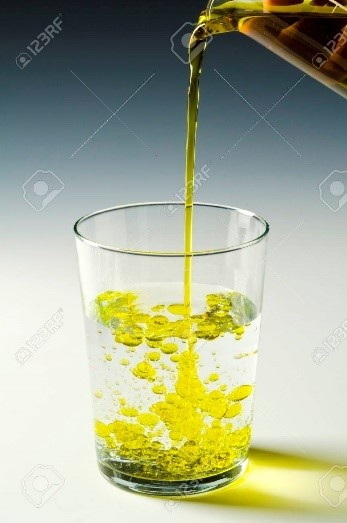
\includegraphics[scale=0.6]{Images/Becher_huile_eau.jpg} & 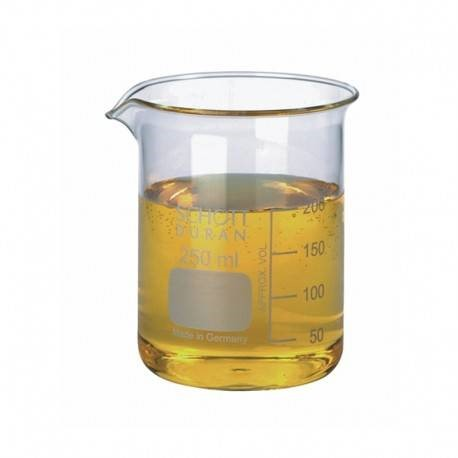
\includegraphics[scale=0.3]{Images/Becher_huile.jpg} & 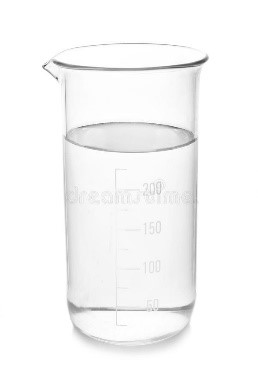
\includegraphics[scale=0.7]{Images/Becher_eau.jpg} & 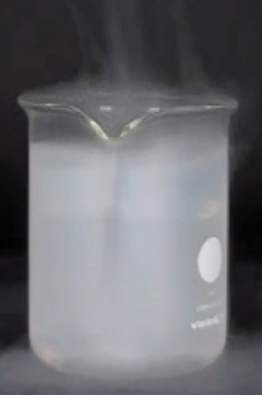
\includegraphics[scale=0.3]{Images/Becher_azote.png} \\
    \hline
    Type de corps & & & & \\
    \hline
    Qualificatif du corps & & & & \\
    \hline
   \end{tabular}
\end{table*}

\section{Identification d'espèces chimiques}
Comment reconnaitre expérimentalement une espèce chimique par rapport à une autre ? On présente dans cette partie quelques éléments qui vont nous permettre de répondre à cette question.

\subsection{Tests chimiques}
\begin{tcolorbox}[colback=red!5!white,colframe=red!75!black,title=\textbf{Tests chimiques à connaître : }]
%\begin{table}
    %\centering
   \begin{tabular}{|C{0.31}|C{0.3}|C{0.31}|}
   \hline
    \cellcolor{blue!25} Espèce chimique à tester & \cellcolor{blue!25} Test & \cellcolor{blue!25} Résultat du test positif \\
    \hline
    Eau (\chemform{H_2O}) & Sulfate de cuivre anhydre (solide blanc)  &  \\
    \hline
    Dioxygène (\chemform{O_2}) & Bûche incandescente &  \\
    \hline
    Dihydrogène (\chemform{H_2}) & Allumette enflammée  &  \\
    \hline 
    Dioxyde de carbone (\chemform{CO_2}) & Eaux de chaux & \\
    \hline
    \end{tabular}
%\end{table}
\end{tcolorbox} 

\subsection{Propriétés physiques}
\subsubsection{La masse volumique}
\begin{tcolorbox}[colback=green!5!white,colframe=green!75!black,title=\textbf{Rappel : masse volumique et densité }]
La masse volumique d'une espèce chimique est :
\begin{equation*}
    \rho = \frac{m}{V}
\end{equation*}
avec m la masse de l'espèce et V son volume. Elle s'exprime en g.cm$^{-3}$.\\
La densité $d$ d'une espèce chimique est le rapport entre la masse volumique de cette substance et la masse volumique de l'eau liquide valant $\rho_{eau}=1$~g.cm$^{-3}$ :
\begin{equation*}
%    d = \frac{\rho_{espece}}{\rho_{eau}}
\end{equation*}
\importantbox{$d$ s'exprime sans unité puisqu'il s'agit d'un rapport entre deux grandeurs physique de même nature.}
\end{tcolorbox}

\begin{tcolorbox}[colback=red!5!white,colframe=red!75!black,title=\textbf{Masse volumique de l'eau: }]
\begin{center}
    $\rho_{eau} = $\gap{................}~kg.m$^{-3}$ ou \gap{.....}~g.cm$^{-3}$. 
\end{center}
\end{tcolorbox}

\begin{tabular}{|c|C{0.06}|C{0.06}|C{0.06}|C{0.1}|C{0.15}|C{0.1}|C{0.1}|}
   \hline
     & Vide & Air & Eau & Glace & Cyclohexane & Bronze & Or \\
    \hline
    $\rho$ (en g.cm$^{-3}$) & 0 & 0,001 & 1,0 & 0,92 & & 7,9 & 19  \\
    \hline
    d & 0 &  & 1 &  &  & & \\
    \hline
    \end{tabular}
\begin{mdframed}[style=autreexo]
\textbf{\bsc{Exercice de cours 3} - Masse volumique du cyclohexane}\\
\textbf{1)} Calculer la masse volumique du cyclohexane sachant qu'un volume de 15~mL a une masse de 11,8~g.\newline \textbf{2)} Le cyclohexane est-il plus dense que l'eau ? \end{mdframed}
\newpage

\subsubsection{Les températures de changement d'état}
\begin{figure}[!htb]
    \centering
    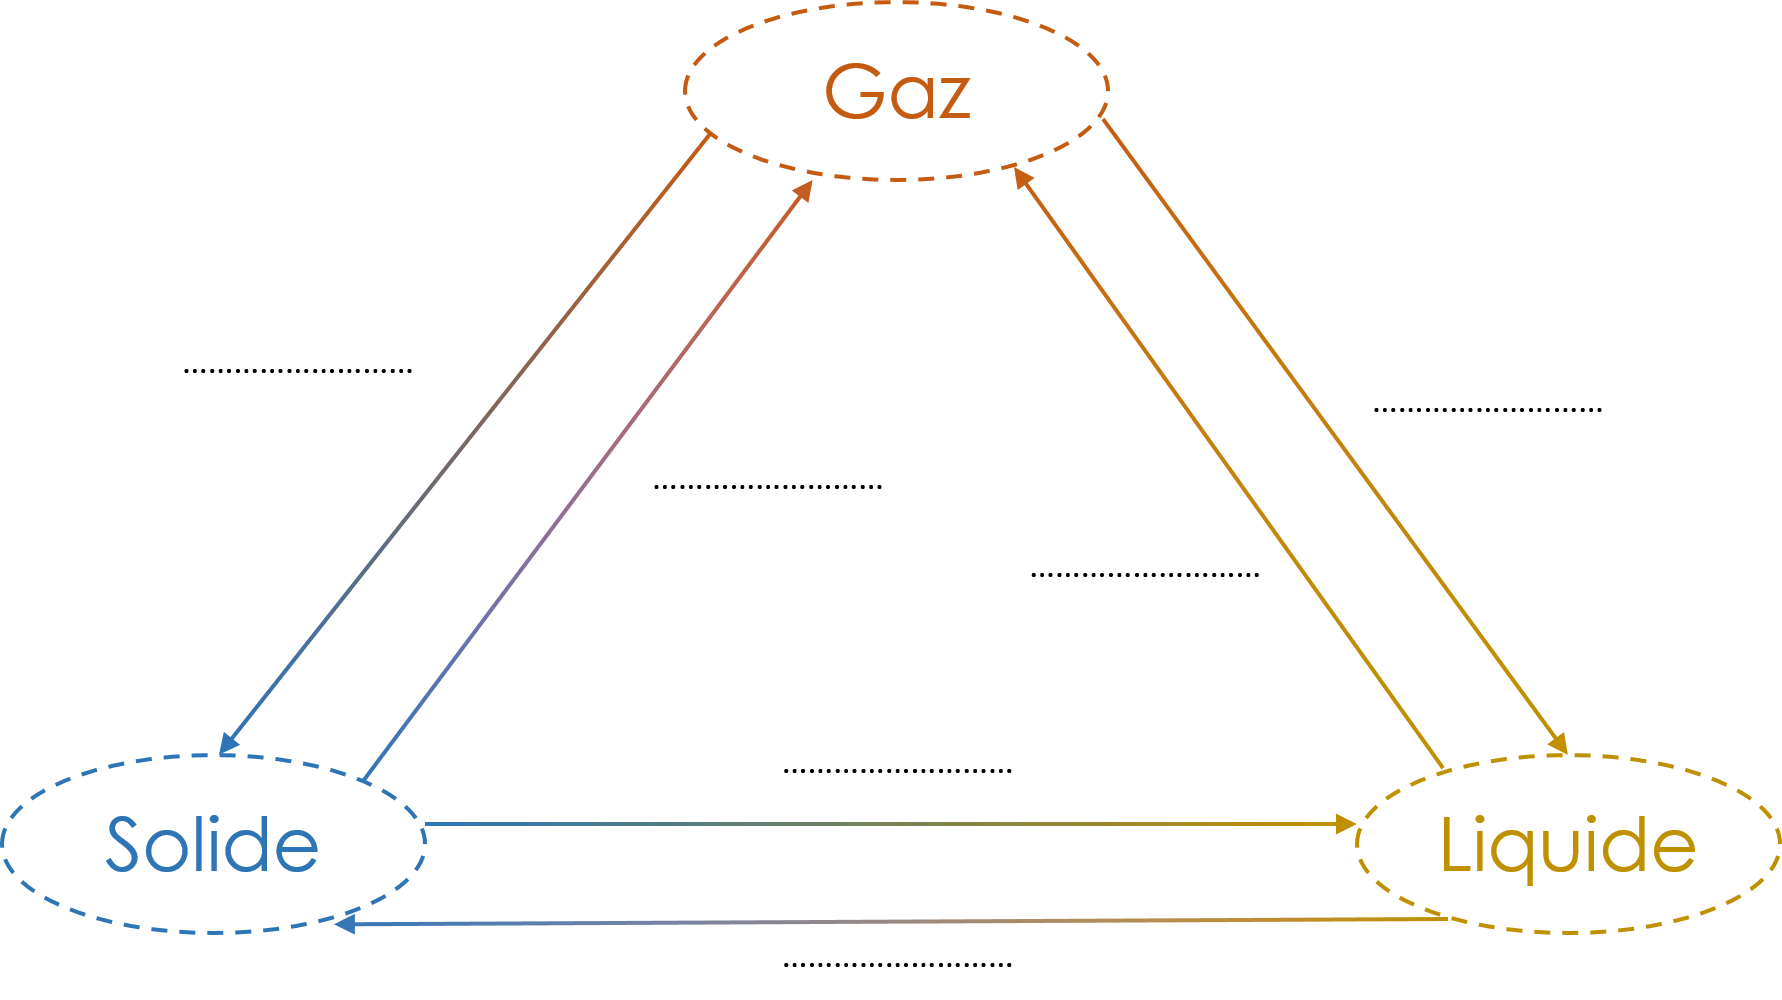
\includegraphics[scale=0.5]{Images/Changement_etat.png}
    \caption{Les changements d'états de la matière}
    \label{fig:enter-label}
\end{figure}
Tout changement d'état \underline{d'un corps pur} s'effectue à une température donnée. Il y a deux définitions importantes à connaître :
\begin{itemize}
    \item On appelle \gap{.....................................................}, notée \gap{.........}, d'une espèce chimique la température \textbf{à partir de laquelle la phase solide de cette espèce commence à fondre},
    \item On appelle \textcolor{red}{température d'ébullition}, notée \gap{.........}, d'une espèce chimique la température \textbf{à partir de laquelle la phase liquide de cette espèce commence à s'évaporer.} 
\end{itemize}
On verra en TP qu'on peut mesurer une température de fusion à l'aide d'un \textcolor{red}{banc Kofler}.

\begin{minipage}{0.6\textwidth}
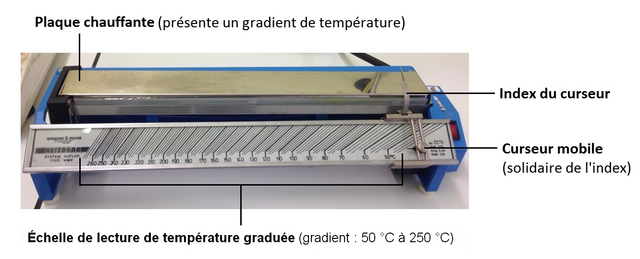
\includegraphics[width=1\textwidth]{Images/Banc_Kofler.png} 
  \end{minipage}
\begin{minipage}{0.4\textwidth}
\underline{\textbf{Exemple à connaitre}} :\newline \`{A} une pression de 1~bar, $\theta_{f}(eau)=$ \gap{.......}$\degreCelsius$ et $\theta_{eb}(eau)=$ \gap{.....}$\degreCelsius$
  \end{minipage}



\newpage

\begin{mdframed}[style=autreexo]
\textbf{\bsc{Exercice de cours 4} - Quel état ?}\\
Dans quel état se trouve l'acide citrique à 0~$\degreCelsius$, à température ambiante (20~$\degreCelsius$) et à 100~$\degreCelsius$.\\
\textit{Données :} $\theta_f=153$~$\degreCelsius$ et $\theta_{eb}=310$~$\degreCelsius$
\end{mdframed}
\vspace{2cm}
\subsection{Chromatograhie sur Couche Mince (CCM)}

\begin{tcolorbox}[colback=green!5!white,colframe=green!75!black,title=\textbf{CCM }, upperbox=invisible]
Une chromatographie sur couche mince est une méthode expérimentale permettant de \textbf{séparer} et \textbf{d'identifier} des éléments chimiques différentes d'un mélange homogène.
\newline
\newline 
\newline
\end{tcolorbox}
Elle repose sur la différence d'affinité des espèces chimiques étudiées pour deux phases :
\begin{itemize}
    \item \textbf{la phase fixe} : la plaque chromatographique composée la plupart du temps de silice,
    \item \textbf{une phase mobile} : l'éluant qui va entraîner les espèces à se séparer le long de la phase fixe.
\end{itemize}

\begin{minipage}[c]{0.4\textwidth}
    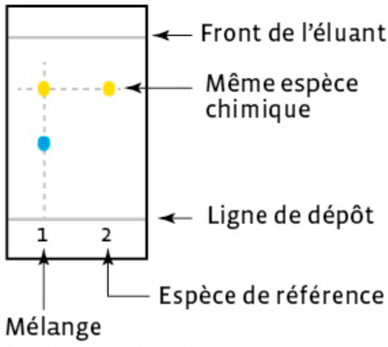
\includegraphics{Images/CCM.png}
\end{minipage}
\begin{minipage}[c]{0.6\textwidth}
    \textbf{Lecture d'un chromatogramme} :
    \begin{itemize}
        \item \underline{Lecture horizontale :} deux tâches situées à la même hauteur correspondent à la même espèce chimique. Ce sont les tâchs jaunes sur la figures de gauche.
        \item  \underline{Lecture verticale :} si un dépôt donne plusieurs tâches (comme c'est le cas sur la figure de gauche), alors il est constitué de plusieurs espèces chimiques : c’est un mélange.
    \end{itemize}
\end{minipage}


\section{Composition d'un mélange}
On vient de voir dans la partie précédente comment identifier une ou plusieurs espèces chimiques en fonction de ses propriétés physico-chimiques. Mais comment donne-t'on la composition d'un mélange ? On introduit ici la proportion volumique et massique d'une espèce dans un mélange.

\subsection{Proportion volumique et massique}

\begin{tcolorbox}[colback=green!5!white,colframe=green!75!black,title=\textbf{Proportion volumique}]
La proportion en volume (ou volumique) d'une espèce dans un mélange est le quotient du volume $V_{E}$ qu'occupe cette espèce par le volume total $V_{tot}$ du mélange :
\newline
\newline
\newline
\newline
avec $V_{E}$ et $V_{tot}$ exprimées dans la même unité (L ou m$^3$ par exemple)\end{tcolorbox}

\begin{tcolorbox}[colback=green!5!white,colframe=green!75!black,title=\textbf{Proportion massique}]
La proportion en masse (ou massique) d'une espèce dans un mélange est le quotient de la masse $m_{E}$ de cette espèce dans le mélange par la masse totale $m_{tot}$ du mélange :
\newline
\newline
\newline
\newline
avec $m_{E}$ et $m_{tot}$ exprimées dans la même unité (g ou kg par exemple).
\end{tcolorbox}

Ces proportions peuvent être exprimées en \% et sont sans unités puisqu'il s'agit d'un rapport en deux grandeurs sans unités.

\subsection{Exemple à connaître : la composition de l'air}
L'air est un mélange de gaz indispensable à la vie sur Terre. Quand il est sec, c'est-à-dire qu'il ne contient pas de vapeur d'eau, voici sa composition :
\begin{figure}[!hbt]
    \centering
    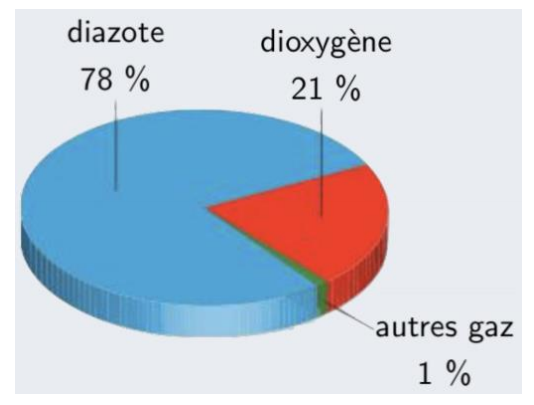
\includegraphics[scale=1]{Images/Composition_air.png}
    \caption{Diagramme de la composition de l'air}
    \label{fig:compo_air}
\end{figure}

\begin{mdframed}[style=autreexo]
\textbf{\bsc{Exercice de cours 5} - Proportion}\\
A partir du diagramme présenté sur la figure, donnez le volume occupé par le diazote et le dioxygène pour un volume d'air total de $100$~L.
\end{mdframed}

  %%\newpage
%$ $
%\newpage

\renewcommand{\thesubsection}{\textcolor{red}{\Roman{section}.\arabic{subsection}}}
\renewcommand{\thesubsubsection}{\textcolor{red}{\Roman{section}.\arabic{subsection}.\alph{subsubsection}}}

\setcounter{section}{0}
\sndEnTeteCoursUn

\begin{center}
\begin{mdframed}[style=titr, leftmargin=60pt, rightmargin=60pt, innertopmargin=7pt, innerbottommargin=7pt, innerrightmargin=8pt, innerleftmargin=8pt]

\begin{center}
\large{\textbf{Chapitre 1: Corps purs et mélanges au quotidien}}
\end{center}

\end{mdframed}
\end{center}
Ce chapitre permet de faire une description de la matière à l'échelle macroscopique (c'est-à-dire à notre échelle). Posons-nous les questions suivantes : Qu'est-ce qu'une espèce chimique ? Comment faire pour en identifier une en laboratoire ? Comment reconnaître un mélange d'une espèce chimique unique ?
%
\begin{tcolorbox}[colback=blue!5!white,colframe=blue!75!black,title=Mots clés du chapitre :]
Corps purs, mélange homogène/hétérogène, masse volumique, températures de changement d'état, solubilité.
\end{tcolorbox}

%

\section{Définitions}

\subsection{Espèces chimiques}

La matière est constituée d'\textcolor{red}{entités chimiques} : les atomes, les molécules, les ions. \`{A} partir de ces entités, on peut définir une \textcolor{red}{espèce chimique} :
\begin{tcolorbox}[colback=green!5!white,colframe=green!75!black,title=\textbf{Espèce chimique}, ]
Elle est composée d'un ensemble d'entités chimiques identiques. Une espèce chimique est caractérisée par :
\begin{itemize}
    \item sa formule chimique : par exemple \chemform{H_2O} pour l'eau,
    \item son aspect : couleur, texture, forme, ...
    \item ses propriétés physiques : température d'ébullition, masse volumique, indice de réfraction, ...
    \item ses propriétés chimiques : réactivité avec d'autres espèces chimiques, ... 
\end{itemize}

\end{tcolorbox}

\begin{mdframed}[style=autreexo]
\textbf{\bsc{Exercice de cours 1} - Espèces chimiques}\\
Donner le type (\textit{atomique}, \textit{moléculaire} ou \textit{ionique}) des espèces chimiques suivantes : hélium (He), eau (H\textsubscript{2}O), chlorure de sodium (Na$^{+}$, Cl$^{-}$).
\end{mdframed}
\textit{Réponse :} He : atomique, H\textsubscript{2}O : moléculaire, (Na$^{+}$, Cl$^{-}$) : ionique.

On distingue alors les \textcolor{red}{corps purs} et les \textcolor{red}{mélanges}.

\subsection{Les corps purs}
\begin{tcolorbox}[colback=green!5!white,colframe=green!75!black,title=\textbf{Corps purs}]
Un corps pur est constitué d'une unique espèce chimique.
\end{tcolorbox}

Les corps purs peuvent être :

\begin{itemize}
    \item \textcolor{red}{simples} : ils sont constitués d'un seul type d'atome. Exemples : le dihydrogène \chemform{H_2}, le charbon \chemform{C}, l'argent \chemform{Ag}.
    \item \textcolor{red}{composés} : ils sont constitués de plusieurs atomes dans des proportions bien définies. Exemples : l'eau \chemform{H_2O}, l'éthanol \chemform{C_2H_6O}, le chlorure de sodium \chemform{(Na^+;Cl^-)}.
\end{itemize}

%%%%%%%%



%
\subsection{Le cas des mélanges}
\begin{tcolorbox}[colback=green!5!white,colframe=green!75!black,title=\textbf{Mélange}]
Un mélange est constitué de plusieurs espèces chimiques différentes.
\end{tcolorbox}
Les mélanges peuvent être :
\begin{itemize}
    \item \textcolor{red}{homogènes} : ils sont constitués d'une seule phase (solide, liquide ou vapeur) indiscernable à l'\oe il nu. Lorsque deux liquides se mélangent l'un avec l'autre, on dit qu'ils sont \textcolor{red}{miscibles}.
    \item \textcolor{red}{hétérogènes} : ils sont constitués de plusieurs phases discernables à l'\oe il nu.
\end{itemize}

\begin{mdframed}[style=autreexo]
\textbf{\bsc{Exercice de cours 2} - Corps purs et mélanges}\\
Pour chaque substance suivante, dire s’il s’agit d’un corps pur simple/complexe ou d’un mélange homogène/hétérogène.
\end{mdframed}
\begin{table*}
    \centering
    \begin{tabular}{|C{0.15}|C{0.15}|c|c|C{0.15}|}
    \hline
    Description & Bécher d'huile et d'eau & Bécher d'huile & Bécher d'eau pure & Bécher d'azote liquide \\
    \hline
    Photographie & 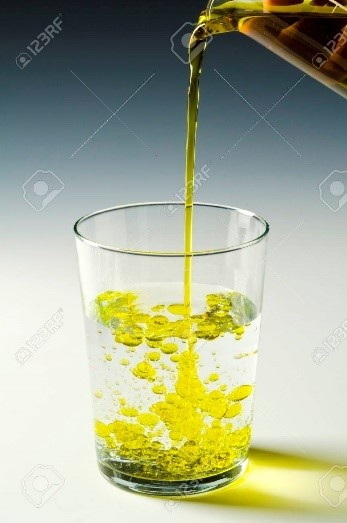
\includegraphics[scale=0.6]{Images/Becher_huile_eau.jpg} & 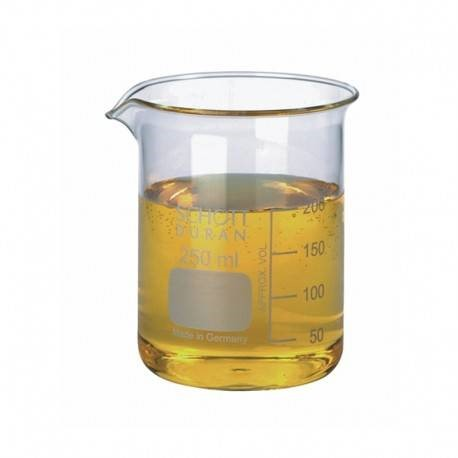
\includegraphics[scale=0.3]{Images/Becher_huile.jpg} & 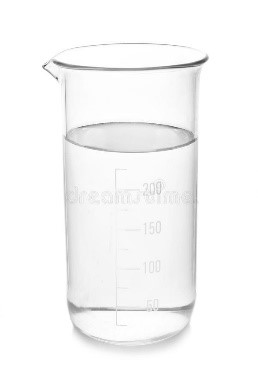
\includegraphics[scale=0.7]{Images/Becher_eau.jpg} & 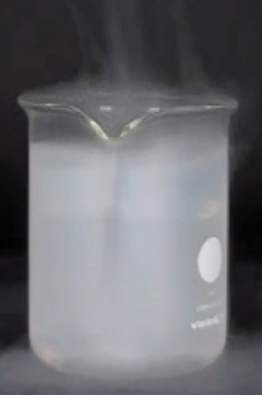
\includegraphics[scale=0.3]{Images/Becher_azote.png} \\
    \hline
    Type de corps & Mélange & Mélange & Corps pur  & Corps pur \\
    \hline
    Qualificatif du corps & Hétérogène & Homogène & Composé & Simple \\
    \hline
   \end{tabular}
\end{table*}

\section{Identification d'espèces chimiques}
Comment reconnaitre expérimentalement une espèce chimique par rapport à une autre ? On présente dans cette partie quelques éléments qui vont nous permettre de répondre à cette question.

\subsection{Tests chimiques}
\begin{tcolorbox}[colback=red!5!white,colframe=red!75!black,title=\textbf{Tests chimiques à connaître : }]
%\begin{table}
    %\centering
   \begin{tabular}{|C{0.31}|C{0.3}|C{0.31}|}
   \hline
    \cellcolor{blue!25} Espèce chimique à tester & \cellcolor{blue!25} Test & \cellcolor{blue!25} Résultat du test positif \\
    \hline
    Eau (\chemform{H_2O}) & Sulfate de cuivre anhydre (solide blanc)  & Apparition d'un précipité bleu \\
    \hline
    Dioxygène (\chemform{O_2}) & Bûche incandescente & La bûche s'enflamme, incandescence ravivée \\
    \hline
    Dihydrogène (\chemform{H_2}) & Allumette enflammée  &  Détonation \\
    \hline 
    Dioxyde de carbone (\chemform{CO_2}) & Eaux de chaux & Eau de chaux troublée, un précipité blanc appararaît \\
    \hline
    \end{tabular}
%\end{table}
\end{tcolorbox} 

\subsection{Propriétés physiques}
\subsubsection{La masse volumique}
\begin{tcolorbox}[colback=green!5!white,colframe=green!75!black,title=\textbf{Rappel : masse volumique et densité }]
La masse volumique d'une espèce chimique est :
\begin{equation*}
    \rho = \frac{m}{V}
\end{equation*}
avec m la masse de l'espèce et V son volume. Elle s'exprime en g.cm$^{-3}$.\\
La densité $d$ d'une espèce chimique est le rapport entre la masse volumique de cette substance et la masse volumique de l'eau liquide valant $\rho_{eau}=1$~g.cm$^{-3}$ :
\begin{equation*}
    d = \frac{\rho_{espece}}{\rho_{eau}}
\end{equation*}
\importantbox{$d$ s'exprime sans unité puisqu'il s'agit d'un rapport entre deux grandeurs physique de même nature.}
\end{tcolorbox}

\begin{tcolorbox}[colback=red!5!white,colframe=red!75!black,title=\textbf{Masse volumique de l'eau: }]
\begin{center}
    $\rho_{eau} = $1000~kg.m$^{-3}$ ou 1~g.cm$^{-3}$. 
\end{center}
\end{tcolorbox}

\begin{tabular}{|c|C{0.06}|C{0.06}|C{0.06}|C{0.1}|C{0.15}|C{0.1}|C{0.1}|}
   \hline
     & Vide & Air & Eau & Glace & Cyclohexane & Bronze & Or \\
    \hline
    $\rho$ (en g.cm$^{-3}$) & 0 & 0,001 & 1,0 & 0,92 & 0,79 & 7,9 & 19  \\
    \hline
    d & 0 & 0,001 & 1,0 & 0,92 & 0,79 & 7,9 & 19 \\
    \hline
    \end{tabular}
\begin{mdframed}[style=autreexo]
\textbf{\bsc{Exercice de cours 3} - Masse volumique du cyclohexane}\\
\textbf{1)} Calculer la masse volumique du cyclohexane sachant qu'un volume de 15~mL a une masse de 11,8~g.\newline \textbf{2)} Le cyclohexane est-il plus dense que l'eau ? \end{mdframed}
\textit{Réponse :} \\
\textbf{1)}. On calcule la masse volumique du cyclohexane à l'aide de la formule du cours : $\rho=\frac{m}{V} = \frac{11,8}{15}=0,79$~g.mL$^{-1}=0,79$ g.cm$^{-3}$.\\
\textbf{2)}. On déduit la densité à l'aide de la formule du cours et de la question 1) : $d=\frac{\rho_{cyclohexane}}{\rho_{eau}}=\frac{0,79}{1,0}=0,79$. Comme $d<1$, le cyclohexane est moins dense que l'eau. 
\newpage

\subsubsection{Les températures de changement d'état}
\begin{figure}[!htb]
    \centering
    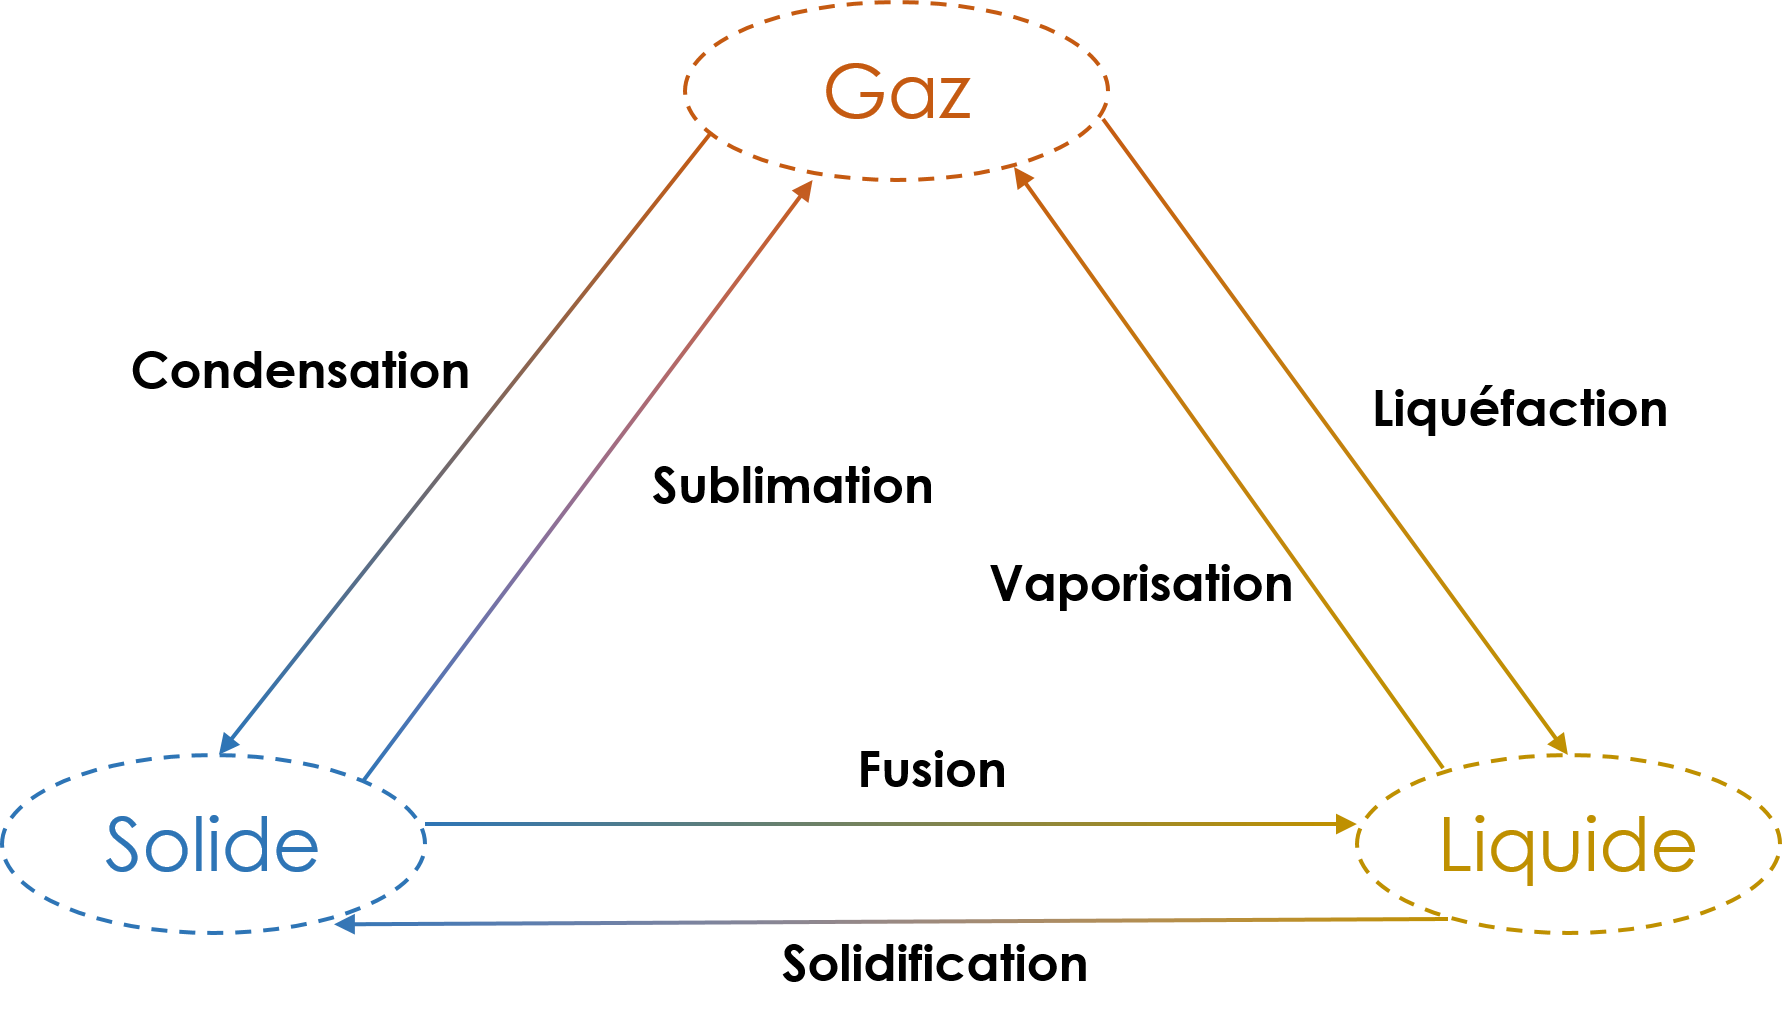
\includegraphics[scale=0.5]{Images/Changement_etat_complet.png}
    \caption{Les changements d'états de la matière}
    \label{fig:enter-label}
\end{figure}
Tout changement d'état \underline{d'un corps pur} s'effectue à une température donnée. Il y a deux définitions importantes à connaître :
\begin{itemize}
    \item On appelle \textcolor{red}{température de fusion}, notée $\theta_f$, d'une espèce chimique la température \textbf{à partir de laquelle la phase solide de cette espèce commence à fondre},
    \item On appelle \textcolor{red}{température d'ébullition}, notée $\theta_{eb}$, d'une espèce chimique la température \textbf{à partir de laquelle la phase liquide de cette espèce commence à s'évaporer.} 
\end{itemize}
On verra en TP qu'on peut mesurer une température de fusion à l'aide d'un \textcolor{red}{banc Kofler}.

\begin{minipage}{0.6\textwidth}
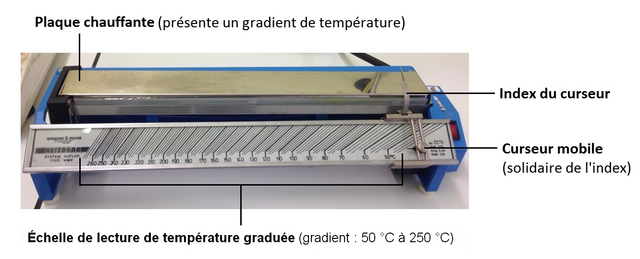
\includegraphics[width=1\textwidth]{Images/Banc_Kofler.png} 
  \end{minipage}
\begin{minipage}{0.4\textwidth}
\underline{\textbf{Exemple à connaitre}} :\newline \`{A} une pression de 1~bar, $\theta_{f}(eau)=0\degreCelsius$ et $\theta_{eb}(eau)=100\degreCelsius$
  \end{minipage}



\newpage

\begin{mdframed}[style=autreexo]
\textbf{\bsc{Exercice de cours 4} - Quel état ?}\\
Dans quel état se trouve l'acide citrique à 0~$\degreCelsius$, à température ambiante (20~$\degreCelsius$) et à 100~$\degreCelsius$.\\
\textit{Données :} $\theta_f=153$~$\degreCelsius$ et $\theta_{eb}=310$~$\degreCelsius$
\end{mdframed}
\textit{Réponse :} Les trois températures 0~$\degreCelsius$, 20~$\degreCelsius$ et 100~$\degreCelsius$ sont inférieures à la température de fusion $\theta_f=153$~$\degreCelsius$ de l'acide citrique. Ce dernier est donc solide à ces températures.

\subsection{Chromatograhie sur Couche Mince (CCM)}

\begin{tcolorbox}[colback=green!5!white,colframe=green!75!black,title=\textbf{CCM }]
Une chromatographie sur couche mince est une méthode expérimentale permettant de \textbf{séparer} et \textbf{d'identifier} des éléments chimiques différentes d'un mélange homogène.
\end{tcolorbox}
Elle repose sur la différence d'affinité des espèces chimiques étudiées pour deux phases :
\begin{itemize}
    \item \textbf{la phase fixe} : la plaque chromatographique composée la plupart du temps de silice,
    \item \textbf{une phase mobile} : l'éluant qui va entraîner les espèces à se séparer le long de la phase fixe.
\end{itemize}

\begin{minipage}[c]{0.4\textwidth}
    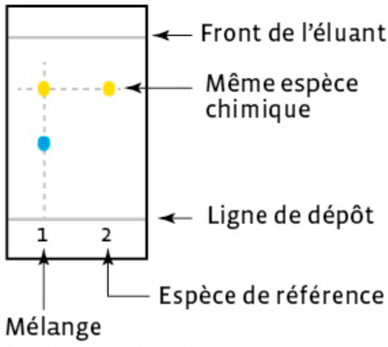
\includegraphics{Images/CCM.png}
\end{minipage}
\begin{minipage}[c]{0.6\textwidth}
    \textbf{Lecture d'un chromatogramme} :
    \begin{itemize}
        \item \underline{Lecture horizontale :} deux tâches situées à la même hauteur correspondent à la même espèce chimique. Ce sont les tâchs jaunes sur la figures de gauche.
        \item  \underline{Lecture verticale :} si un dépôt donne plusieurs tâches (comme c'est le cas sur la figure de gauche), alors il est constitué de plusieurs espèces chimiques : c’est un mélange.
    \end{itemize}
\end{minipage}

\section{Composition d'un mélange}
On vient de voir dans la partie précédente comment identifier une ou plusieurs espèces chimiques en fonction de ses propriétés physico-chimiques. Mais comment donne-t'on la composition d'un mélange ? On introduit ici la proportion volumique et massique d'une espèce dans un mélange.

\subsection{Proportion volumique et massique}

\begin{tcolorbox}[colback=green!5!white,colframe=green!75!black,title=\textbf{Proportion volumique}]
La proportion en volume (ou volumique), notée $x_V$ d'une espèce dans un mélange est le quotient du volume $V_{E}$ qu'occupe cette espèce par le volume total $V_{tot}$ du mélange :
\begin{equation*}
    x_V=\frac{V_E}{V_{tot}}
\end{equation*}
avec $V_{E}$ et $V_{tot}$ exprimées dans la même unité (L ou m$^3$ par exemple)
\end{tcolorbox}

\begin{tcolorbox}[colback=green!5!white,colframe=green!75!black,title=\textbf{Proportion massique}]
La proportion en masse (ou massique), notée $x_m$, d'une espèce dans un mélange est le quotient de la masse $m_{E}$ de cette espèce dans le mélange par la masse totale $m_{tot}$ du mélange :
\begin{equation*}
    x_m=\frac{m_E}{m_{tot}}
\end{equation*}
avec $m_{E}$ et $m_{tot}$ exprimées dans la même unité (g ou kg par exemple).
\end{tcolorbox}

Ces proportions peuvent être exprimées en \% et sont sans unités puisqu'il s'agit d'un rapport en deux grandeurs sans unités.

\subsection{Exemple à connaître : la composition de l'air}
L'air est un mélange de gaz indispensable à la vie sur Terre. Quand il est sec, c'est-à-dire qu'il ne contient pas de vapeur d'eau, voici sa composition :
\begin{figure}[!hbt]
    \centering
    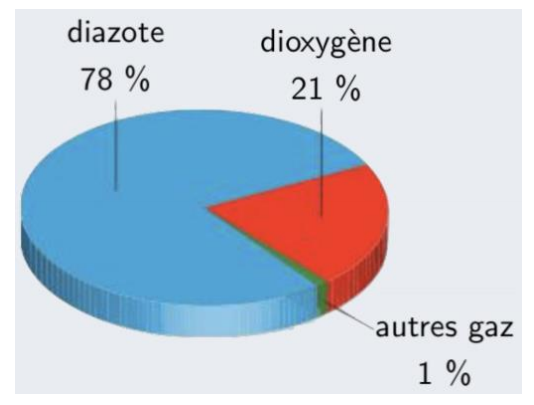
\includegraphics[scale=0.5]{Images/Composition_air.png}
    \caption{Diagramme de la composition de l'air}
    \label{fig:compo_air}
\end{figure}

\begin{mdframed}[style=autreexo]
\textbf{\bsc{Exercice de cours 5} - Proportion}\\
A partir du diagramme présenté sur la figure, donnez le volume occupé par le diazote et le dioxygène pour un volume d'air total de $100$~L.
\end{mdframed}
\textit{Réponse :} Diazote : $V_{N_2}=78\%*100=78$~L. Dioxygène : $V_{O_2}=21\%*100=21$~L.



  %%%%%%%%%% Exercices %%%%%%%%
  %\renewcommand{\thesubsection}{\textcolor{red}{\Roman{section}.\arabic{subsection}}}
\renewcommand{\thesubsubsection}{\textcolor{red}{\Roman{section}.\arabic{subsection}.\alph{subsubsection}}}

\setcounter{section}{0}
\enTeteExo{1}

\begin{center}
\begin{mdframed}[style=titr, leftmargin=60pt, rightmargin=60pt, innertopmargin=7pt, innerbottommargin=7pt, innerrightmargin=8pt, innerleftmargin=8pt]

\begin{center}
\large{\textbf{Feuille d'exercices du Chapitre 1}}
\end{center}

\end{mdframed}
\end{center}

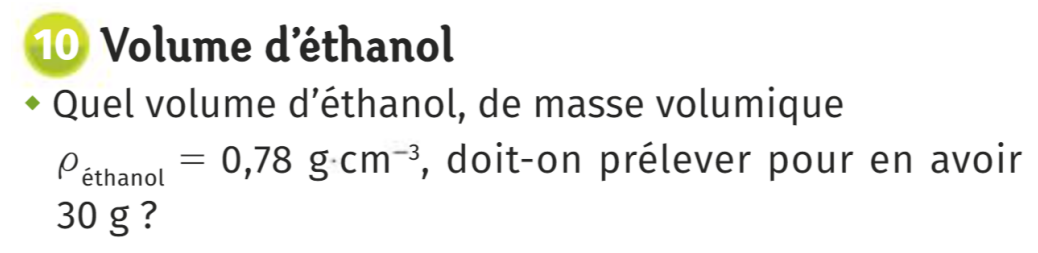
\includegraphics[scale=0.9]{Images/Exo_1_Chap1.png}
\vspace{1cm}

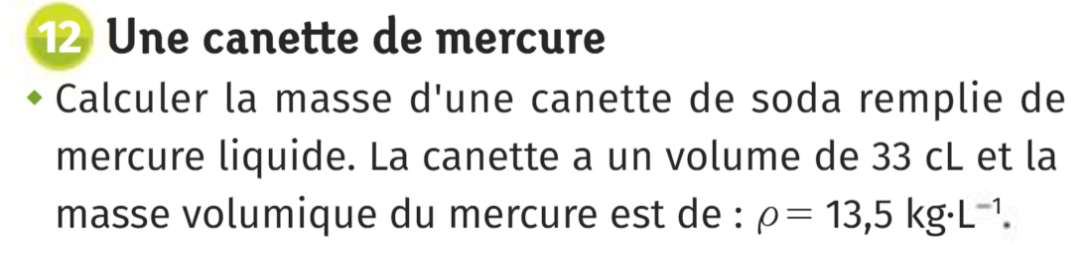
\includegraphics[scale=0.9]{Images/Exo_2_Chap1.png}
\vspace{1cm}

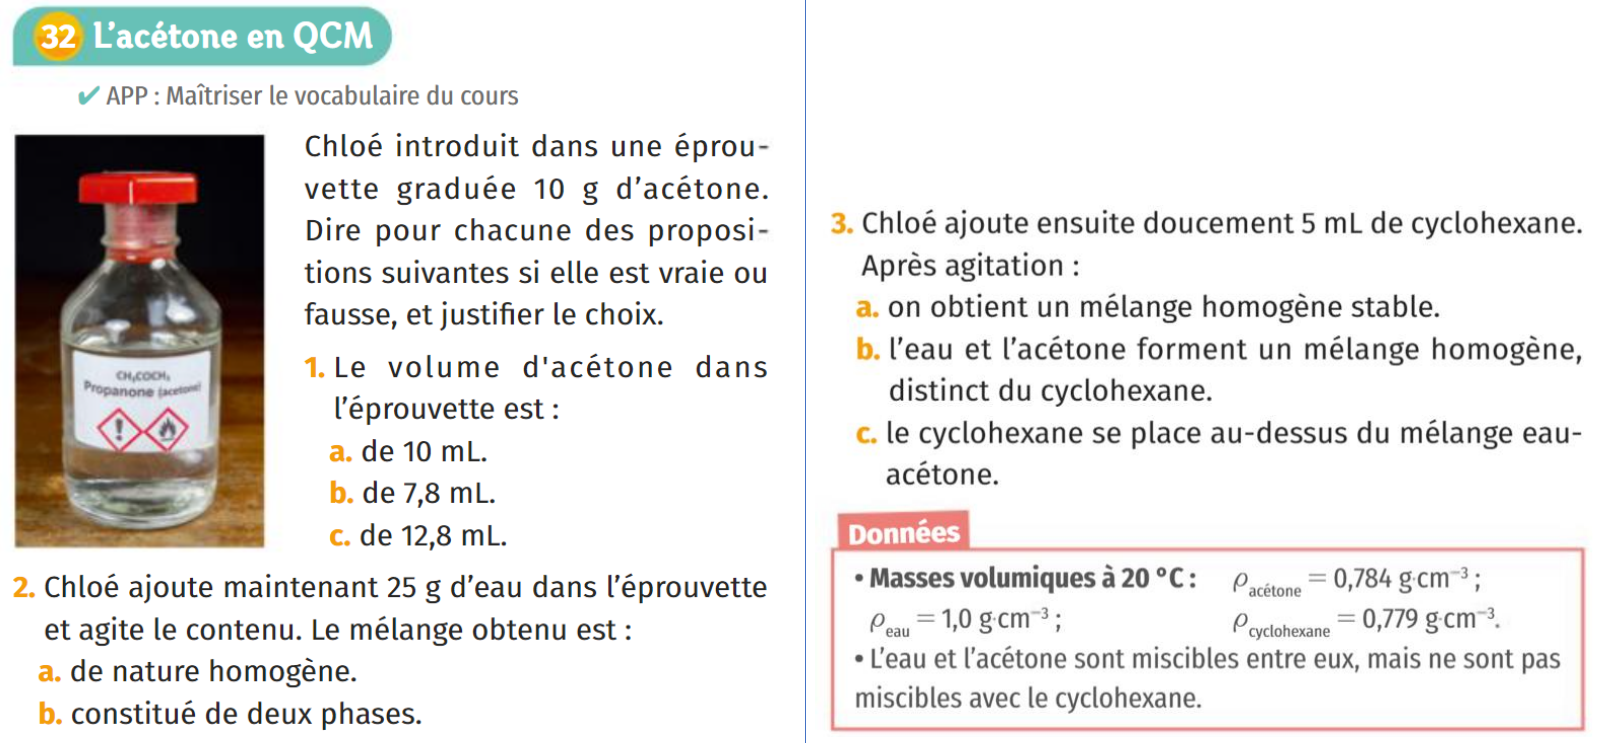
\includegraphics[scale=0.7]{Images/Exo_32_Chap1.png}
\vspace{1cm}

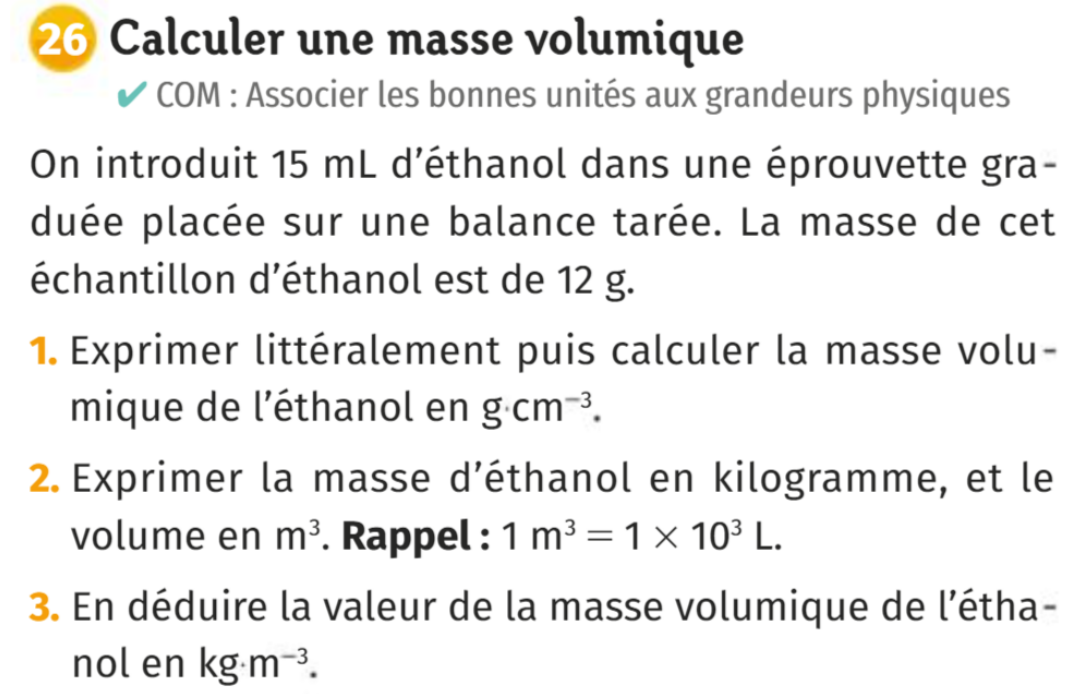
\includegraphics[scale=0.8]{Images/Exo_3_Chap1.png}
\vspace{1cm}

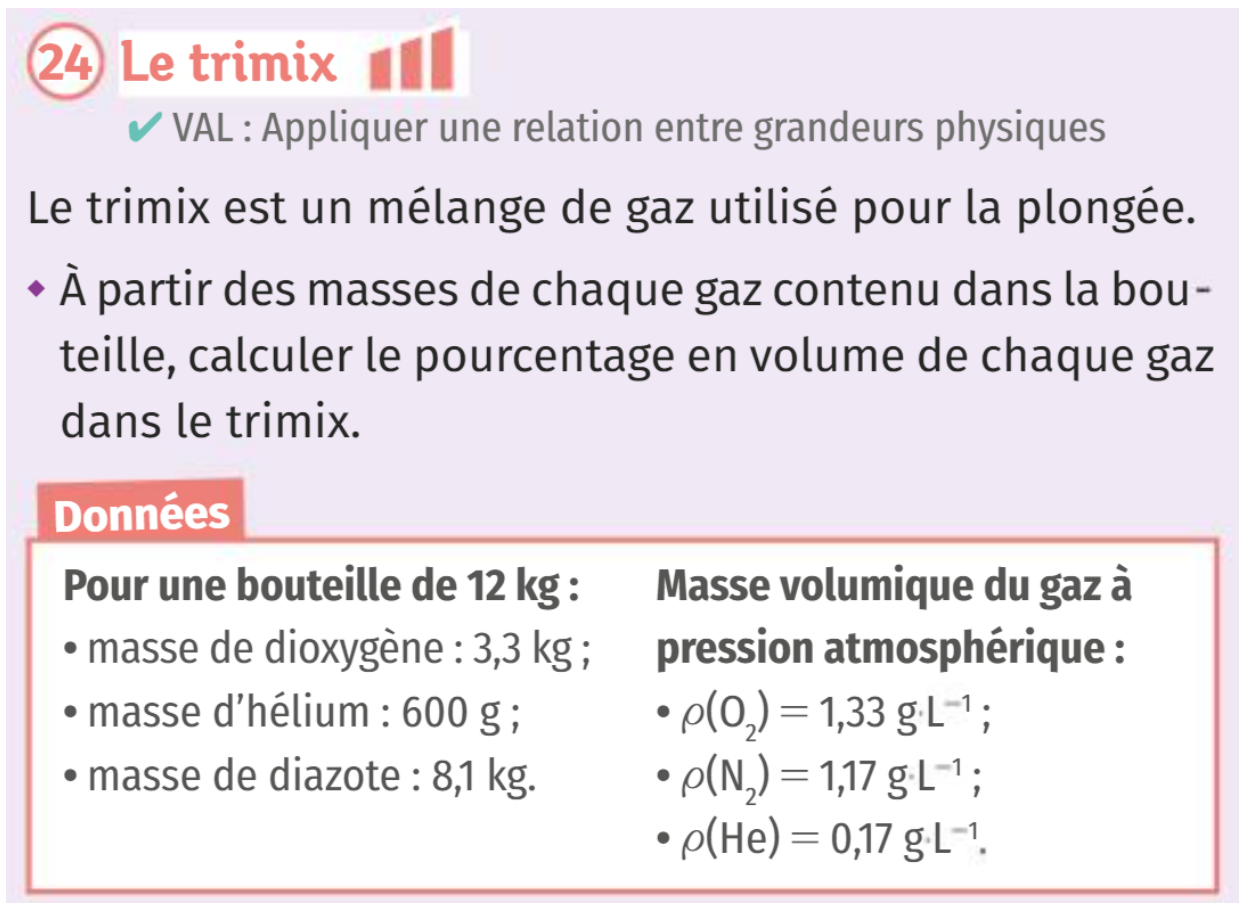
\includegraphics[scale=0.6]{Images/Exo_24_Chap1.png}
\vspace{1cm}

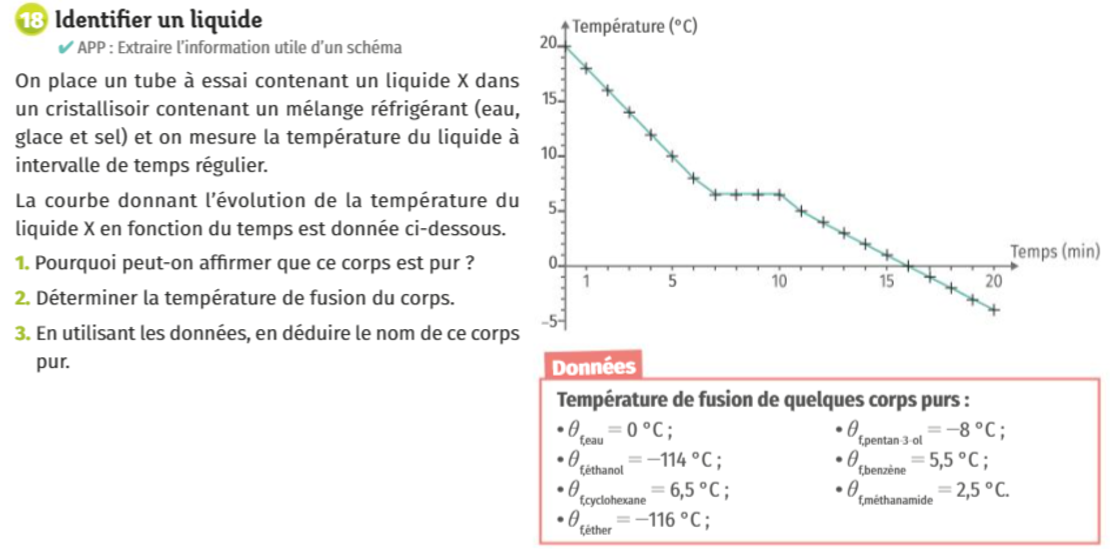
\includegraphics[scale=1]{Images/Exo_18_Chap1.png}



  %%%%%%%%%% Activités %%%%%%%%
  %\renewcommand{\thesubsection}{\textcolor{red}{\Roman{section}.\arabic{subsection}}}
\renewcommand{\thesubsubsection}{\textcolor{red}{\Roman{section}.\arabic{subsection}.\alph{subsubsection}}}

\setcounter{section}{0}
\setcounter{document}{0}
\sndEnTeteActUn

\begin{center}
\begin{mdframed}[style=titr, leftmargin=60pt, rightmargin=60pt, innertopmargin=7pt, innerbottommargin=7pt, innerrightmargin=8pt, innerleftmargin=8pt]

\begin{center}
\large{\textbf{Activité 1 : Composition d'un mélange eau-huile}}
\end{center}

\end{mdframed}
\end{center}
\begin{Large}{\textbf{Q : Quelle est la proportion volumique et massique de l'huile et de l'eau présent dans l'éprouvette graduée sur le bureau du professeur ?}} \end{Large} 
\begin{mdframed}[style=autreexo]
\textbf{\bsc{Consignes :}}
\begin{itemize}
    \item Lever la main si vous souhaitez vous déplacer,
    \item Lever la main si vous souhaitez un indice,
    \item Vous pouvez travailler en binôme \textbf{\underline{uniquement}} avec votre voisin de table,
    \item Vous pouvez rendre le travail à la fin de l'heure si vous améliorer votre note d'interrogation.
   
\end{itemize}
\end{mdframed}

\begin{doc}{Lecture d'un volume sur la verrerie}

\begin{wrapfigure}{r}{0.3\textwidth}
\vspace{-2cm}
    \centering
      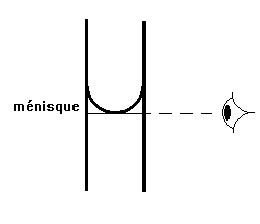
\includegraphics[width=0.27\textwidth]{Images/Lecture_Verrerie.png}
  \end{wrapfigure}
  Lorsqu'on verse un liquide dans une pièce de verrerie (éprouvette, tube à essai, etc), l se forme un ménisque qui va perturber la mesure du volume sur cette verrerie. Pour lire le volume occupé par un liquide, il faut positionner son \oe il sur le bas du ménisque.%En 1775, Antoine Lavoisier réalise une expérience qui lui permet de déterminer la composition de l’air.
%Son expérience est résumée dans la vidéo suivante : \url{https://ladigitale.dev/digiplay/#/v/6305f2f7b8fd4}.\\
%D’après Lavoisier, l’air est constitué de deux gaz : le dioxygène et le diazote. Le volume du gaz initialement
%présent dans la cloche est de 0,80 L d’air. À la fin de l’expérience, le volume du gaz qui n’a pas réagi avec le
%mercure (c’est-à-dire le diazote) est de 0,66 L.}
\end{doc}

\begin{doc}{Proportion volumique ou massique d’une espèce dans un mélange}
Pour décrire la composition d’un mélange, on indique la proportion (ou le pourcentage) de chaque espèce chimique constituant le mélange. On peut choisir d’utiliser la proportion massique notée $x_m$, ou la proportion volumique notée $x_V$ :
\begin{align*}
    x_m &= \frac{m_{\text{espèce}}}{m_{\text{totale}}} & x_V & = \frac{V_{\text{espèce}}}{V_{\text{totale}}}\\
\end{align*}
Ces deux grandeurs s'expriment en général en \%.
\end{doc}

\begin{doc}{Données utiles}
La masse volumique de l'huile est :
\begin{equation*}
    \rho_{huile} = 0,92 \text{~g.cm$^{-3}$}
    \end{equation*}
\end{doc}

  %\renewcommand{\thesubsection}{\textcolor{red}{\Roman{section}.\arabic{subsection}}}
\renewcommand{\thesubsubsection}{\textcolor{red}{\Roman{section}.\arabic{subsection}.\alph{subsubsection}}}

\setcounter{section}{0}
\setcounter{document}{0}
\sndEnTeteActUn

\begin{center}
\begin{mdframed}[style=titr, leftmargin=60pt, rightmargin=60pt, innertopmargin=7pt, innerbottommargin=7pt, innerrightmargin=8pt, innerleftmargin=8pt]

\begin{center}
\large{\textbf{Activité 1 : Composition d'un mélange eau-huile - \textbf{Correction}}}
\end{center}

\end{mdframed}
\end{center}
\begin{Large}{\textbf{Q : Quelle est la proportion volumique et massique de l'huile et de l'eau présent dans l'éprouvette graduée sur le bureau du professeur ?}} \end{Large}
\newline

\`{A} la lecture sur l'éprouvette graduée, on lisait :
\begin{enumerate}
    \item $V_{huile}=15$~mL,
    \item $V_{eau}=30$~mL,
    \item $V_{Tot}= 45$~mL $=V_{huile}+V_{eau}$
\end{enumerate}

\section{Calcul de la proportion volumique de l'huile et de l'eau}
On en déduit directement la proportion volumique pour chaque espèce :
\begin{enumerate}
    \item $x_V(huile)=\frac{V_{huile}}{V_{Tot}}=\frac{15}{45}=33\%$
    \item $x_V(eau)=\frac{V_{eau}}{V_{Tot}}=\frac{30}{45}=67\%$
    \item \textcolor{red}{On vérifie bien que $x_V(huile)+x_V(eau)=100\%$}
\end{enumerate}

\section{Calcul de la proportion massique de l'huile et de l'eau}
Maintenant pour calculer la proportion massique de chaque espèce chimique, on doit d'abord calculer la masse de chaque espèce chimique. \\

\textbf{\underline{D'après le cours}}, la relation qui lie la masse et le volume est celle de la masse volumique à savoir :
\begin{equation*}
    \rho_{\text{espèce}} = \frac{m_{\text{(espèce)}}}{V_{\text{espèce}}}
\end{equation*}

On en déduit donc :
\begin{enumerate}
    \item $m_{\text{eau}}=\rho_{\text{eau}}\times V_{\text{eau}}=1,0~\text{g/mL}\times 30~\text{mL}=30$~g. \textcolor{red}{On ne garde que deux chiffres significatifs au résultat},
    \item $m_{\text{huile}}=\rho_{\text{huile}}\times V_{\text{eau}}=0,92~\text{g/mL}\times 15~\text{mL}=14$~g. \textcolor{red}{On ne garde que deux chiffres significatifs au résultat}
    \item $m_{Tot}=m_{\text{huile}}+m_{\text{eau}}=44$~g.
\end{enumerate}

On en déduit donc d'après le Document 2 la proportion massique des deux espèces :
\begin{align*}
    x_m(eau)&=\frac{m_{\text{eau}}}{m_{Tot}}=\frac{30}{44}=68\% & x_m(huile)&=\frac{m_{\text{eau}}}{m_{Tot}}=\frac{14}{44}=32\% 
\end{align*}
\textcolor{red}{On vérifie bien que $x_m(huile)+x_m(eau)=100\%$}

  %%%%%%%%%% TP %%%%%%%%%%%%%%%
  %%\newpage
%$ $
%\newpage

\renewcommand{\thesubsection}{\textcolor{red}{\Roman{section}.\arabic{subsection}}}
\renewcommand{\thesubsubsection}{\textcolor{red}{\Roman{section}.\arabic{subsection}.\alph{subsubsection}}}

\setcounter{section}{0}
\sndEnTeteTPUn

\begin{center}
\begin{mdframed}[style=titr, leftmargin=60pt, rightmargin=60pt, innertopmargin=7pt, innerbottommargin=7pt, innerrightmargin=8pt, innerleftmargin=8pt]

\begin{center}
\large{\textbf{TP 1 : Identification d'espèces par tests chimiques}}
\end{center}

\end{mdframed}
\end{center}



\begin{tcolorbox}[colback=blue!5!white,colframe=blue!75!black,title=Objectifs de la séance :]
\begin{itemize}
    \item Respecter les règles de sécurité d’un laboratoire de chimie.
    \item Mettre en œuvre les tests chimiques de présence d’eau, de dihydrogène, de dioxygène et de dioxyde de carbone.

\end{itemize}
\end{tcolorbox}

\begin{tcolorbox}[colback=orange!5!white,colframe=orange!75!black,title= Scénario:]
La majorité des liquides et des gaz mis en jeu lors des expériences de chimie sont incolores. Le chimiste a pourtant besoin de les distinguer : il utilise pour cela des tests chimiques.
\end{tcolorbox}

\section*{Documents mis à disposition}

\begin{doc}{Quelques tests chimiques vus au collège}
    \begin{center}
        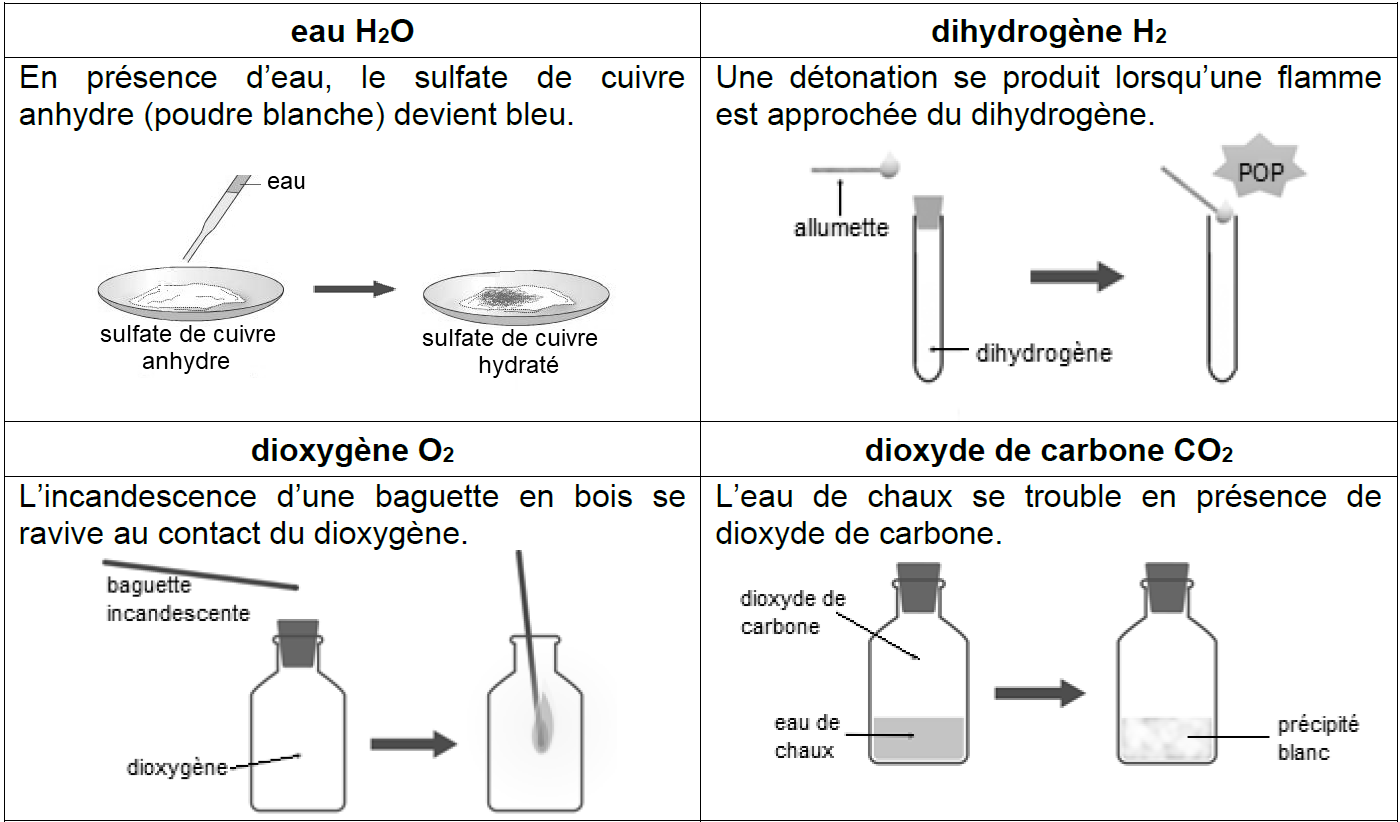
\includegraphics[scale=0.46]{Images/Tests_chimiques.png}
    \end{center}
\end{doc}

\begin{doc}{Pictogrammes de sécurité des produits utilisés lors du TP}
    \begin{minipage}{0.5\linewidth}
        
        \begin{center}
            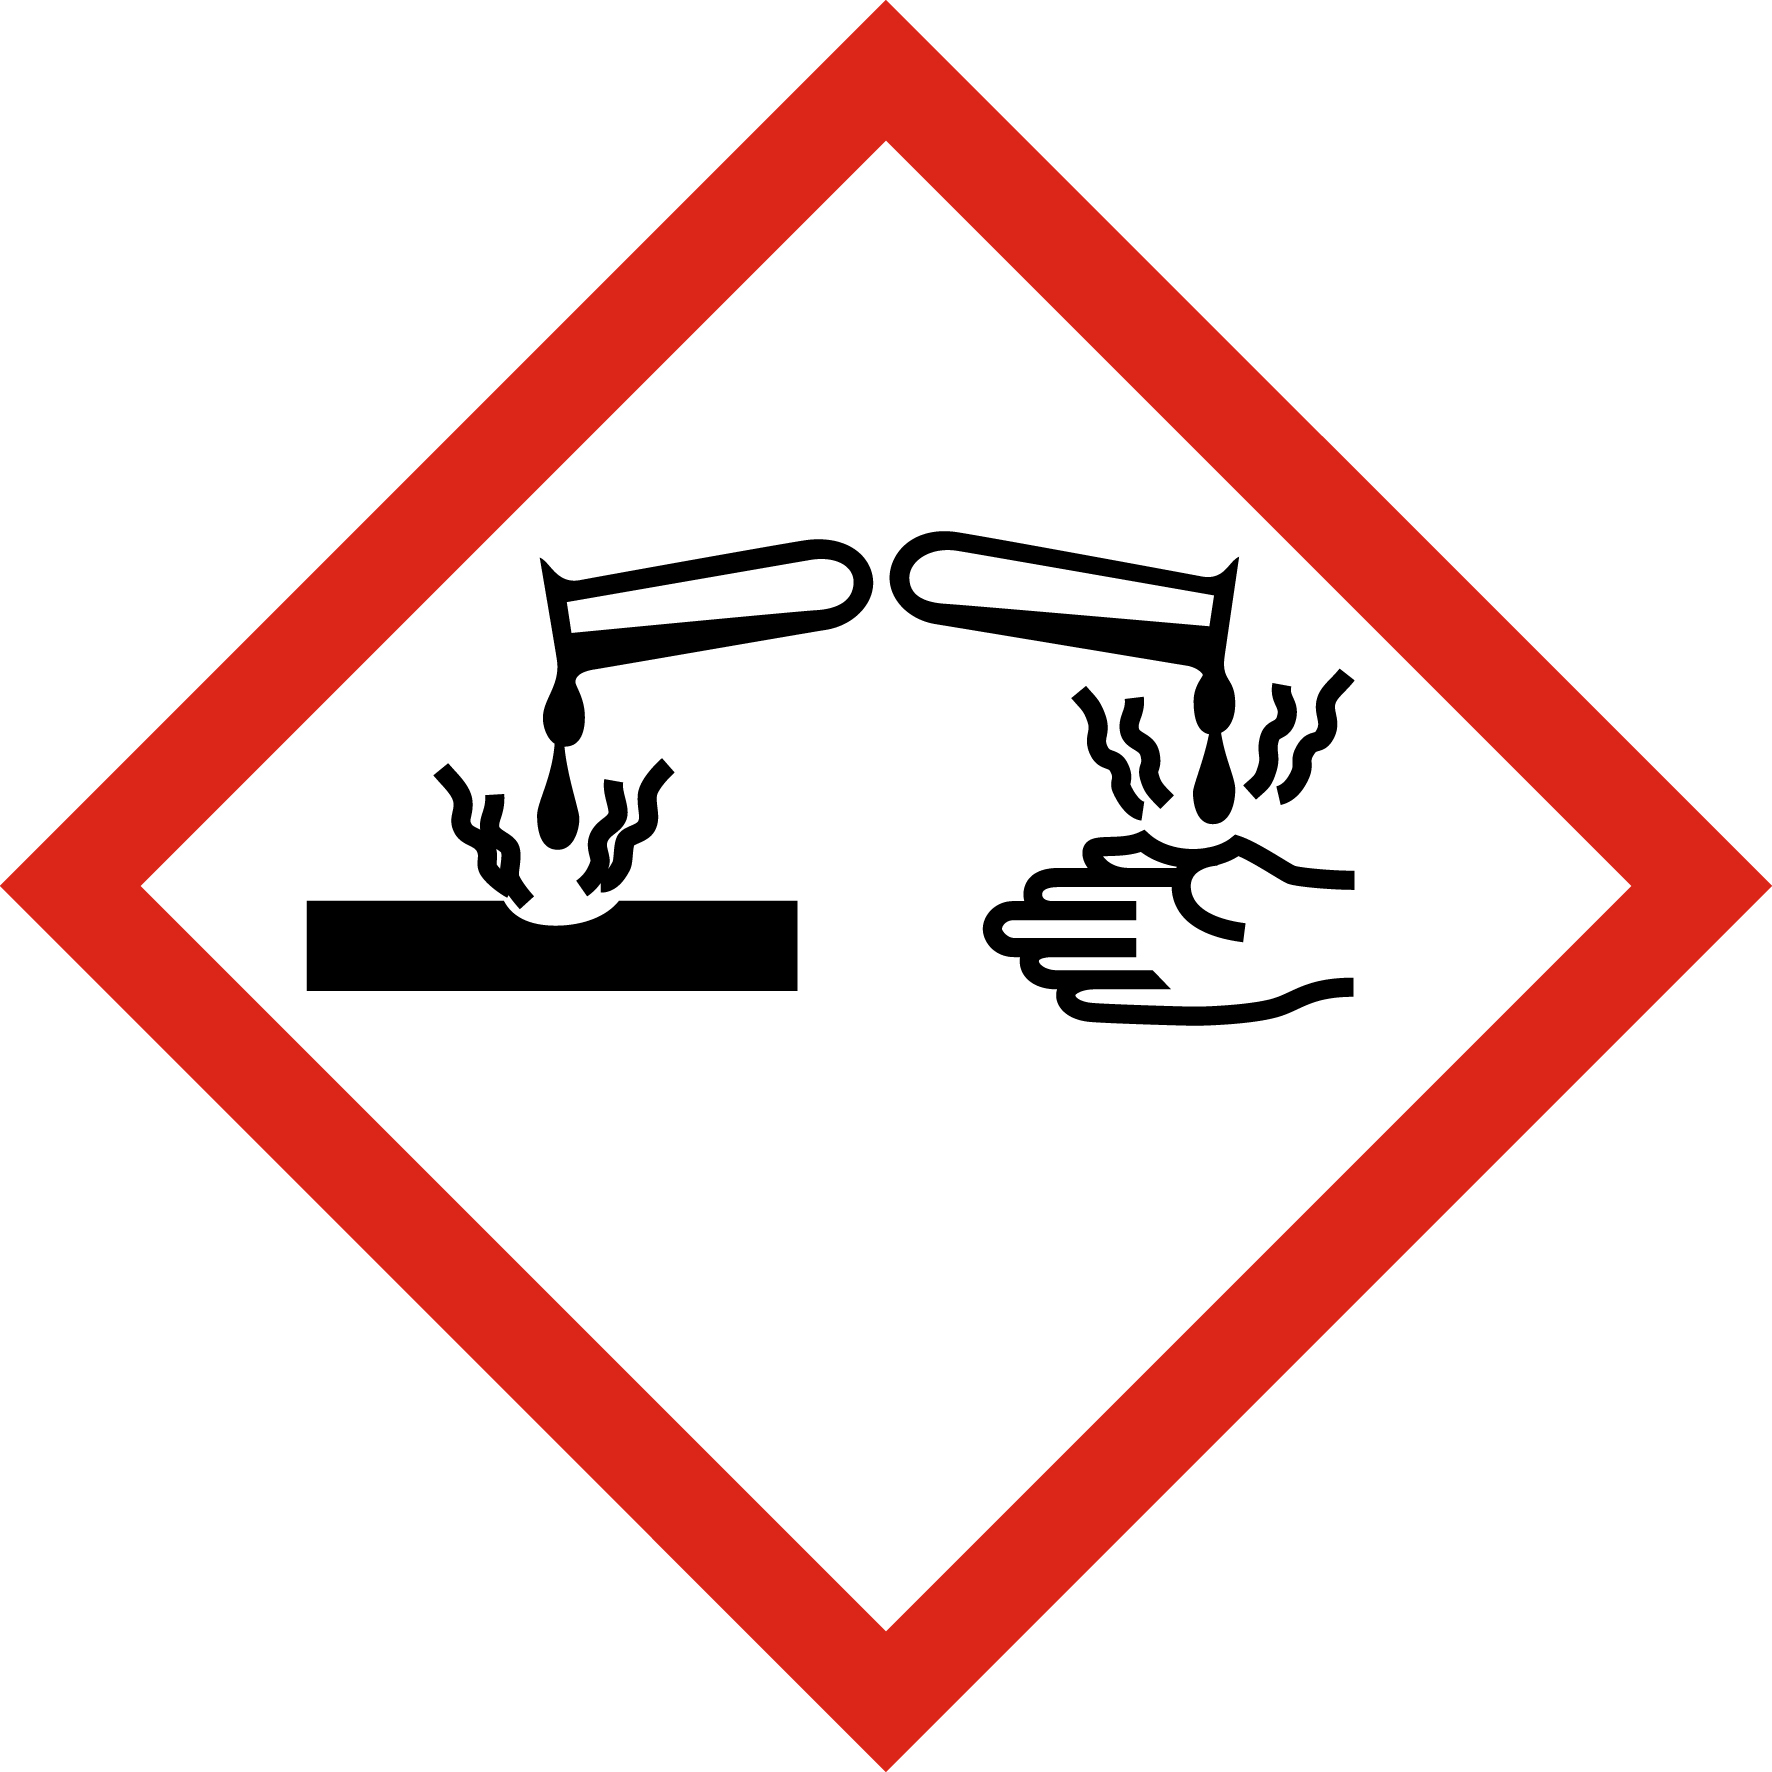
\includegraphics[scale=0.3]{Images/SGH05_Corrosion.jpg}
        \end{center}
        \begin{itemize}
            \item Solution d'acide chlorhydrique (\chemform{H^+_{(aq)}+Cl^-_{(aq)}})
            \item solution de chlorure de fer III (\chemform{Fe^{3+}_{(aq)}+3Cl^-_{(aq)}})
            \item eau oxygénée \chemform{H_2O_2}
        \end{itemize}
        
    \end{minipage}
    \begin{minipage}{0.5\linewidth}\vspace{-1.8cm}
    \begin{center}
        
\includegraphics[scale=0.3]{Images/SGH07_PointExclamation.jpg}
    \end{center}
    \begin{itemize}
            \item eau de chaux (\chemform{Ca^{2+}_{(aq)}+HO^-_{(aq)}})
            \item sulfate de cuivre anhydride \chemform{CuSO_4(s)}
    \end{itemize}
    \end{minipage}
    \vspace{1cm}
    
    \begin{large}
        \ding{52}
    \end{large}Pour s'approprier les pictogrammes de sécurité : \url{https://learningapps.org/display?v=pz0yp6isn23} 
\end{doc}

\begin{doc}{Protocoles expérimentaux}
\begin{minipage}{\linewidth}
\begin{center}
    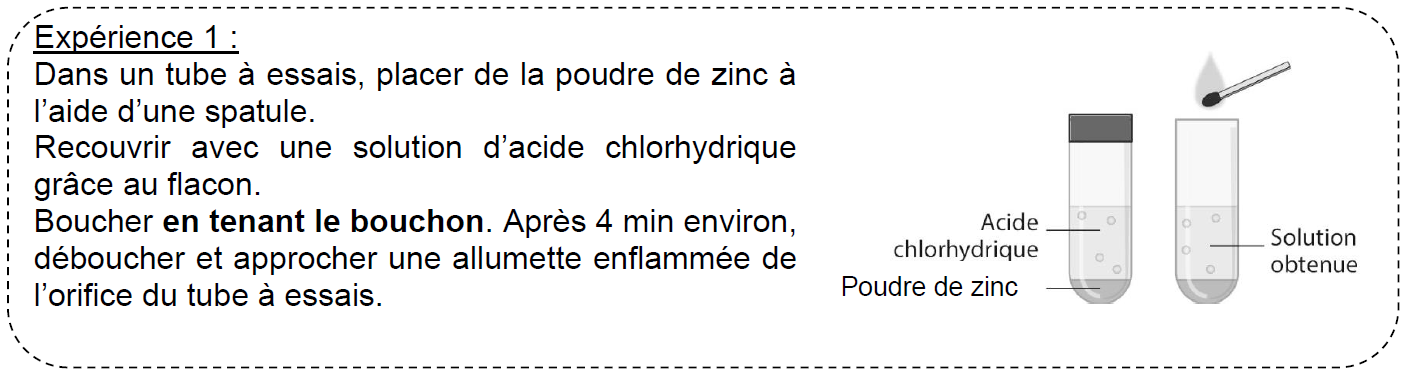
\includegraphics[scale=0.46]{Images/Exp_H2.png}
\end{center}
\end{minipage}
\begin{minipage}{\linewidth}
\begin{center}
    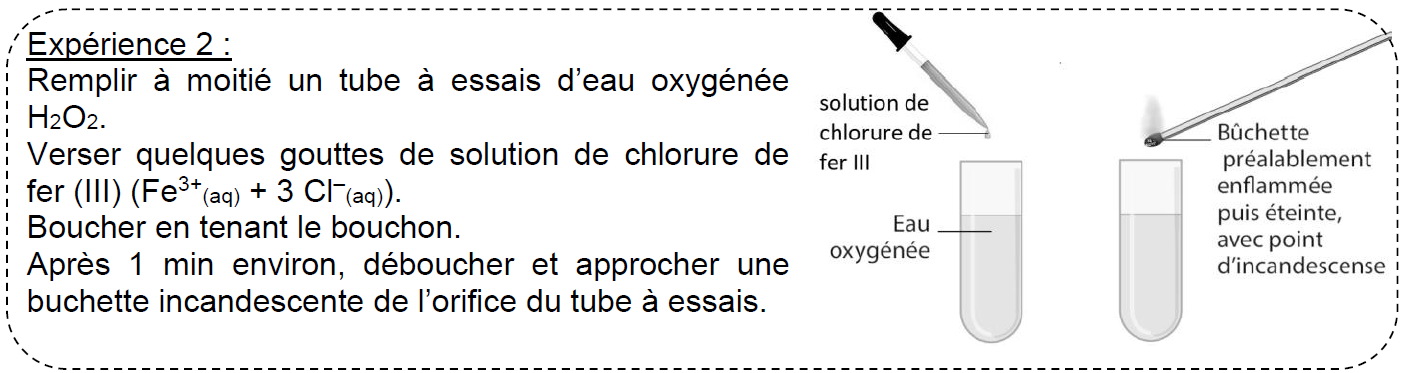
\includegraphics[scale=0.46]{Images/Exp_O2.png}
\end{center}
\end{minipage}
\begin{minipage}{\linewidth}
\begin{center}
    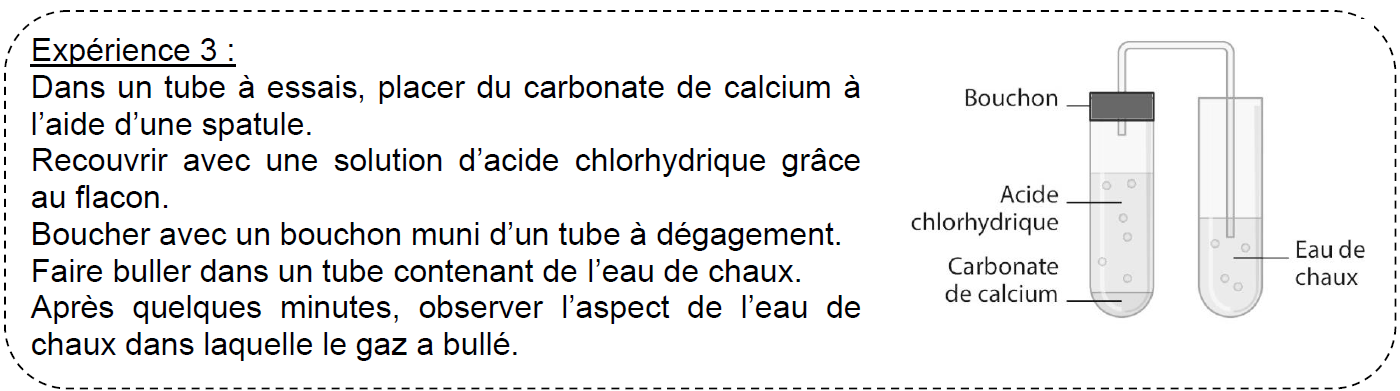
\includegraphics[scale=0.46]{Images/Exp_CO2.png}
\end{center}
\end{minipage}
\end{doc}

\begin{mdframed}[style=autreexo]
\textbf{\bsc{Liste du matériel}}
\begin{itemize}
    \item un flacon contenant de la poudre de zinc ;
    \item un flacon contenant une solution d’acide chlorhydrique ;
    \item un flacon contenant de l’eau oxygénée \chemform{H_2O_2};
    \item un flacon contenant une solution de chlorure de fer III ;
    \item un flacon contenant du carbonate de calcium en poudre ;
    \item une pissette d'éthanol à 95\% ;
    \item une solution de glycérol ;
    \item une spatule ;
    \item une boite d’allumettes ;
    \item une bûchette en bois ;
    \item des tubes à essais et leur support ;
    \item des bouchons pour tubes à essais ;
    \item un tube à dégagement et un bouchon pour tube à essais adapté ;
    \item une coupelle ;
    \item des béchers ;
    \item des pipettes simples ;
	\item des gants et des lunettes de protection.
 
\end{itemize}
\end{mdframed}

\newpage

\begin{Large}
    \textbf{\textcolor{red}{Travail à effectuer :}}
\end{Large}
\\
\begin{enumerate}
    \item Allumer votre ordinateur. Aller sur le site \url{https://learningapps.org/display?v=pz0yp6isn23} et effectuer l'activité.
    \item À l’aide du document 2, expliquer pourquoi il sera obligatoire de porter des gants, en plus de la blouse et des lunettes de protection, tout au long de l’activité.
    \item Réaliser les trois expériences du document 3 et noter vos observations expérimentales.
    \item À l’aide du document 1, identifier pour chacune des expériences du document 3 le gaz libéré.
    \item Compléter le tableau du document de cours avec vos observations
    \item On dispose de deux solutions : une d'éthanol commerciale et une de glycérol. Proposer un protocole permettant de déterminer si ces solutions contiennent de l'eau.
    \item Appeler le professeur pour valider ce protocole.
    \item Mettre en \oe uvre le protocole et noter vos observations expérimentales.
    \item La solution d'éthanol est-elle pure ? Que veut dire \og Solution d'éthanol à 95\% \fg ?
\end{enumerate}

\textit{Bonus pour les plus rapides : calculer la masse d'éthanol contenue dans la bouteille suivante : }

\begin{minipage}{0.5\textwidth}
\centering
    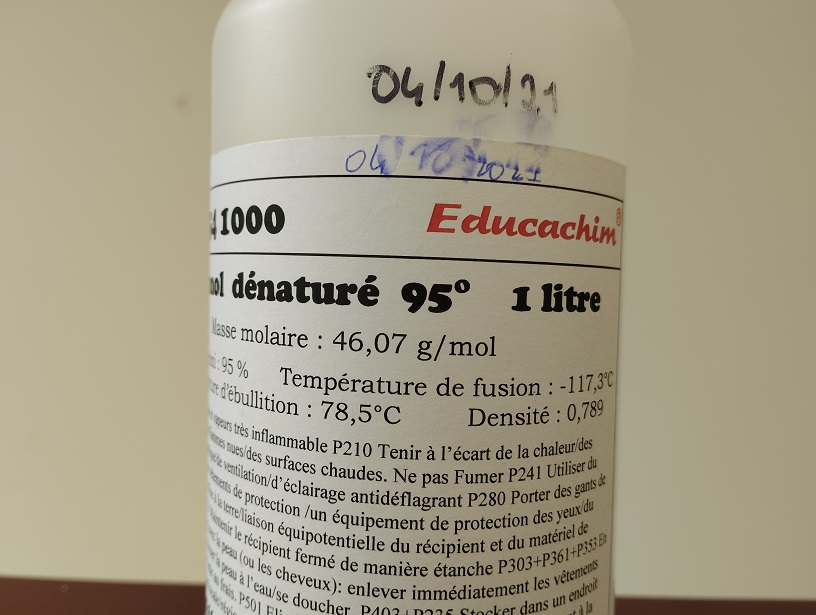
\includegraphics[scale=0.3]{Images/Bouteille_ethanol.jpg}
\end{minipage}
\begin{minipage}{0.5\textwidth}
\centering
    
\includegraphics[scale=0.3]{Images/qrcode_picto.png}
    \\
    QR-code pour les pictogrammes de sécurité.
\end{minipage}


  %%\newpage
%$ $
%\newpage

\renewcommand{\thesubsection}{\textcolor{red}{\Roman{section}.\arabic{subsection}}}
\renewcommand{\thesubsubsection}{\textcolor{red}{\Roman{section}.\arabic{subsection}.\alph{subsubsection}}}

\setcounter{section}{0}
\setcounter{document}{0}
\sndEnTeteTPDeux

\begin{center}
\begin{mdframed}[style=titr, leftmargin=60pt, rightmargin=60pt, innertopmargin=7pt, innerbottommargin=7pt, innerrightmargin=8pt, innerleftmargin=8pt]

\begin{center}
\large{\textbf{TP 2 : Mais qui a pollué la Seine ?}}
\end{center}

\end{mdframed}
\end{center}



\begin{tcolorbox}[colback=blue!5!white,colframe=blue!75!black,title=Objectifs de la séance :]
\begin{itemize}
    \item Mesurer une température de changement d'état,
    \item Réaliser une chromatographie sur couche mince,
\end{itemize}
\end{tcolorbox}

\begin{tcolorbox}[colback=orange!5!white,colframe=orange!75!black,title= Scénario:]
\og Le 5 août dernier, une compétition-test pré-JO de natation en eaux libres dans la Seine avait dû être annulée en raison de la pollution du fleuve.\fg 
\begin{flushright}
    \textit{Source : RadioFrance, le 16 août 2023}
\end{flushright}
\begin{large}
    \ding{43}
\end{large} Une grande usine est suspectée d’avoir déversé des milliers de litres de produits chimiques dans la Seine. Une équipe de scientifique a permis par évaporation d'isoler un solide blanc présent dans l'eau et un colorant. Vous avez pour mission de déterminer qui a déversé ces produits chimiques.
\end{tcolorbox}
\begin{center}
    \textbf{\textcolor{red}{Vous présenterez en fin de TP votre rapport d'enquêteur au professeur.}}
\end{center}

\section{Analyse d'une espèce solide}

\begin{doc}{Utilisation du banc Kofler}
Le banc Kofler est une plaque chauffante présentant un gradient de température, c’est à dire une augmentation progressive de la température de droite (température ambiante) à gauche (environ 250$\degreCelsius$-300$\degreCelsius$ selon les bancs). \textbf{Le banc Kofler permet de déterminer la température de fusion d’une espèce chimique}.
\begin{center}
    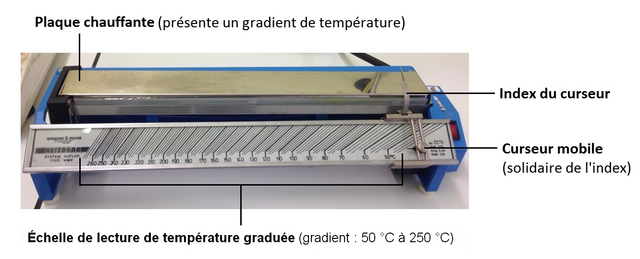
\includegraphics[scale=0.65]{Images/Banc_Kofler.png} 
\end{center}

Avant toute utilisation, le banc doit être étalonné (c’est-à-dire calibré). Voici les étapes d'utilisation du banc Kofler :
\begin{enumerate}
    \item \textbf{Etalonnage} \textit{(réalisé par le professeur)} : une très petite quantité de l’espèce étalon est déposée sur la partie froide du banc. On déplace ensuite cette quantité vers la partie chaude jusqu’à observer sa fusion. Le curseur de température est alors ajusté pour faire correspondre son index avec la température de l’étalon. Le banc doit ensuite être essuyé, pour enlever tous les résidus.
    \item \textbf{Mesure :} Comme lors de l’étalonnage, une petite quantité de l’espèce est déposée sur la partie froide du banc. On déplace ensuite cette quantité vers la partie chaude jusqu’à observer sa fusion. On lit à l’aide du curseur la température de fusion.
\end{enumerate}
Voici le lien d'une vidéo sur l'utilisation du banc : \url{https://ladigitale.dev/digiview/#/v/630614d1b4375}\\
\importantbox{Ne pas utiliser de gants lors de l'utilisation du banc Kofler !}
\end{doc}

\begin{doc}{Schéma des entreprises en bordure de la Seine}
\begin{center}
    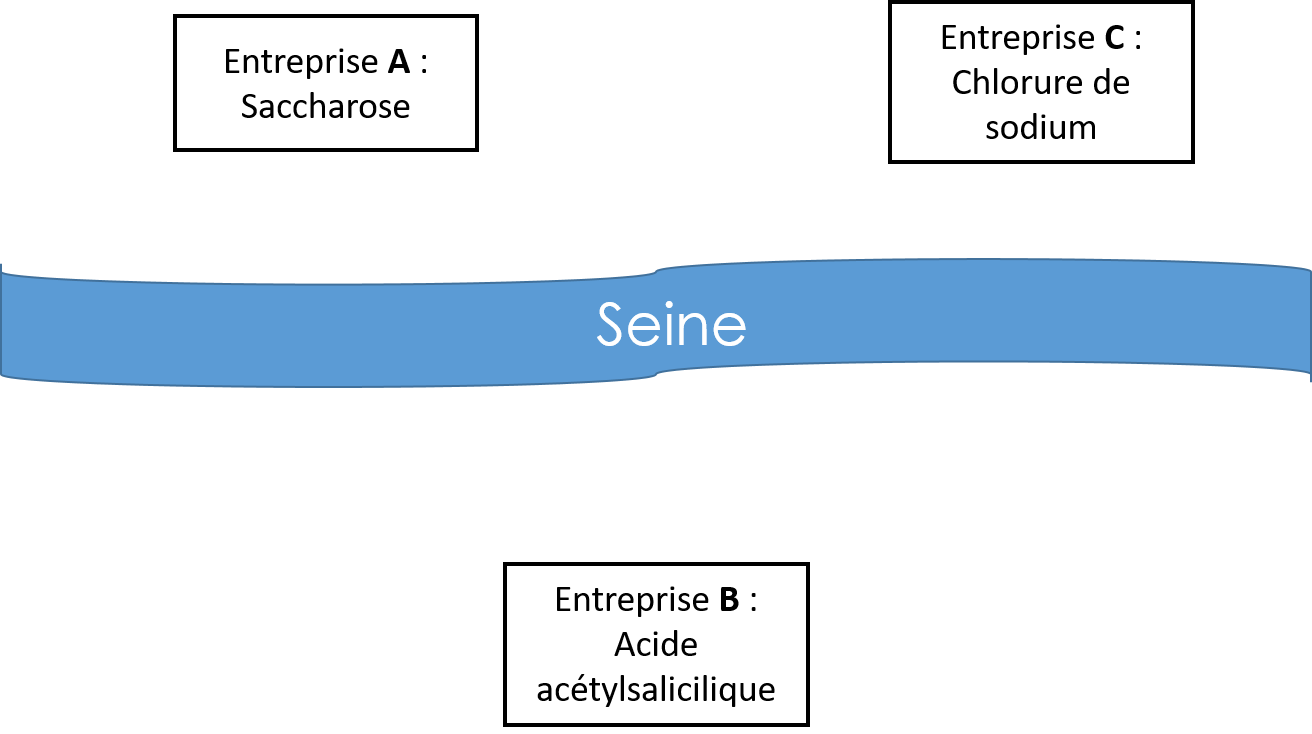
\includegraphics[scale=0.5]{Images/Entreprise.png}
\end{center}
\end{doc}
\newpage
\begin{doc}{Fiche technique des trois produits chimiques fabriqués par les entreprises}
\newline
    \begin{tabular}{|C{0.4}|C{0.1}|C{0.2}|C{0.2}|}
    \hline
     & Chlorure de sodium & Saccharose & Acide acétylsalycilique \\
    \hline
    Température de fusion $T_{f}$ \newline (en $\degreCelsius$) & 801 & 185,5 & 135 \\
    \hline
    Température d'ébullition $T_{eb}$ \newline (en $\degreCelsius$) & 1465 & Décomposition & Se décompose à 140 $\degreCelsius$ \\
    \hline
    Masse volumique (en g.cm$^{-3}$) & 2,16 & 1,59 & 1,4 \\
    \hline
    \end{tabular}
\end{doc}

\textbf{Vous souhaitez déterminer l’entreprise d’où provient la poudre retrouvée sur la victime pour en déduire ainsi le lieu du crime.}\\
A l’aide des documents :
\begin{enumerate}
    \item Trouver et rédiger le protocole à mettre en place
    \item Réaliser l’expérience
    \item Déterminer le lieu du crime en justifiant,
    \item \textit{(Bonus)} Proposer une autre technique qui aurait pu permettre de déterminer le lieu du crime
\end{enumerate}

\section{Analyse d'un colorant}
Maintenant que vous avez découvert le lieu du crime, les enquêteurs penchent sur deux suspects : le Professeur Violet qui utilise les colorants E102 et E131 et le Docteur Orchidée qui utilise le colorant E133.\\

\begin{doc}{Mettre en place une Chromatographie sur Couche Mince (CCM)}
Protocole expérimental :
    \begin{itemize}
        \item Introduire l’éluant (eau + éthanol) dans la cuve à chromatographie (sur environ 0,5 cm de hauteur). Fermer la cuve avec son couvercle pour la saturer en vapeurs d’éluant.
        \item Tracer, au crayon, sur le papier filtre la ligne de dépôt à 1,5 cm du bord inférieur. Placer, en les espaçant d’au moins 1 cm, une marque par dépôt à effectuer (ici 4 dépôts, \textbf{notez les sur le papier filtre !}),
        \item Déposer les échantillons à analyser à l’aide d’un tube capillaire. Un dépôt pour le feutre, un dépôt pour la tâche, un dépôt pour l’encre.
        \item Introduire la plaque dans la cuve (attention, la ligne de dépôt et les échantillons ne doivent pas être immergés dans l’éluant !) 
        \item Retirer la plaque à chromatographie de la cuve lorsque l’éluant a migré jusqu’à atteindre 1 cm du bord supérieur. Tracer au crayon le front de solvant.
    \end{itemize}
Une animation pour réaliser une CCM est disponible à cette adresse \url{https://ladigitale.dev/digiplay/#/v/63061cea42993} 
\end{doc}
%\qrcode{https://ladigitale.dev/digiplay/#/v/63061cea42993}
\begin{doc}{Analyse comparative d'un ou plusieurs chromatogrammes}
\begin{wrapfigure}{r}{0.4\textwidth}
\vspace{-1cm}
    \centering
      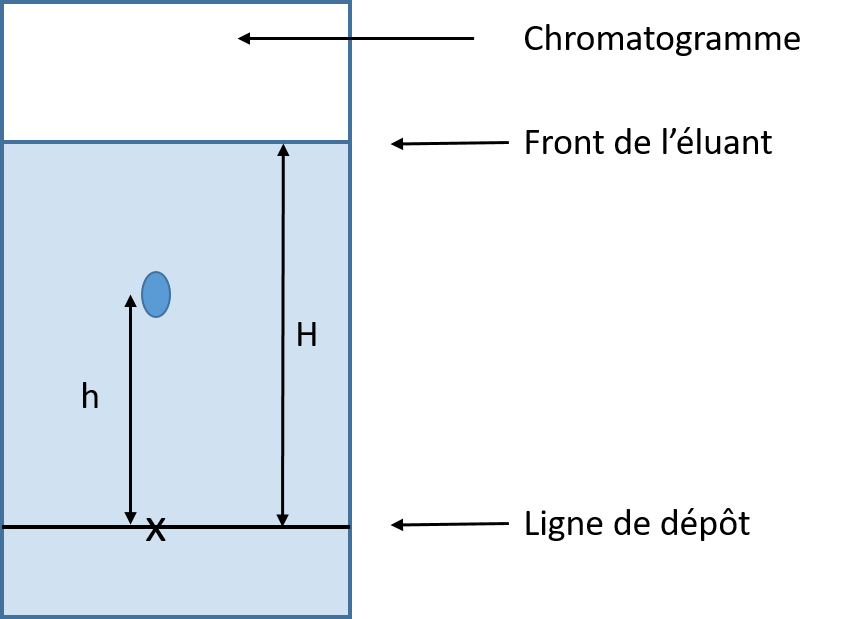
\includegraphics[width=0.4\textwidth]{Images/Chromatogramme.png}
  \end{wrapfigure}
    Le rapport frontal (noté $R_f$) se calcule à l'aide de la formule suivante :
\begin{equation*}
    R_f = \frac{h}{H}
\end{equation*}
avec $h$ la distance parcourue par l'espèce chimique, $H$ la distance parcourue par le front de l'éluant.\\
\textbf{Si deux espèces chimiques ont le même rapport frontal, alors elles sont identiques.}

\end{doc}



\begin{mdframed}[style=autreexo]
\textbf{\bsc{Liste du matériel}}
\begin{itemize}
    \item tube capillaire,
    \item flacon de colorant E133 ;
    \item flacon de colorant E102 ;
    \item flacon de colorant E131 ;
    \item papier filtre ;
    \item cuve chromatographique avec éluant ;
\end{itemize}
\end{mdframed}
A l’aide des documents :
\begin{enumerate}
    \item À l’aide d’un schéma, présenter les résultats de la CCM,
    \item Interpréter les résultats de la CCM,
    \item Déterminer le coupable.
\end{enumerate}
  %%\newpage
%$ $
%\newpage

\renewcommand{\thesubsection}{\textcolor{red}{\Roman{section}.\arabic{subsection}}}
\renewcommand{\thesubsubsection}{\textcolor{red}{\Roman{section}.\arabic{subsection}.\alph{subsubsection}}}

\setcounter{section}{0}
\setcounter{document}{0}
\sndEnTeteTPTrois

\begin{center}
\begin{mdframed}[style=titr, leftmargin=60pt, rightmargin=60pt, innertopmargin=7pt, innerbottommargin=7pt, innerrightmargin=8pt, innerleftmargin=8pt]

\begin{center}
\large{\textbf{TP 3 : Détermination de la composition d'un mélange : l'alcool pharmaceutique}}
\end{center}

\end{mdframed}
\end{center}



\begin{tcolorbox}[colback=blue!5!white,colframe=blue!75!black,title=Objectifs de la séance :]
Mesurer des volumes et des masses pour estimer la composition de mélanges.
\end{tcolorbox}

\begin{tcolorbox}[colback=orange!5!white,colframe=orange!75!black,title= Scénario:]
Un pharmacien vend de l’alcool pharmaceutique (mélange eau-éthanol), qui sert de désinfectant notamment pour le matériel médical. L’étiquette d’un flacon d’alcool pharmaceutique porte la mention de sa composition. Le pharmacien aimerait s’assurer que cette indication est correcte.
\end{tcolorbox}

\section{Documents mis à disposition}

\begin{multicols}{2}
    \begin{doc}{Flacon d'alcool pharmaceutique}
\begin{center}
    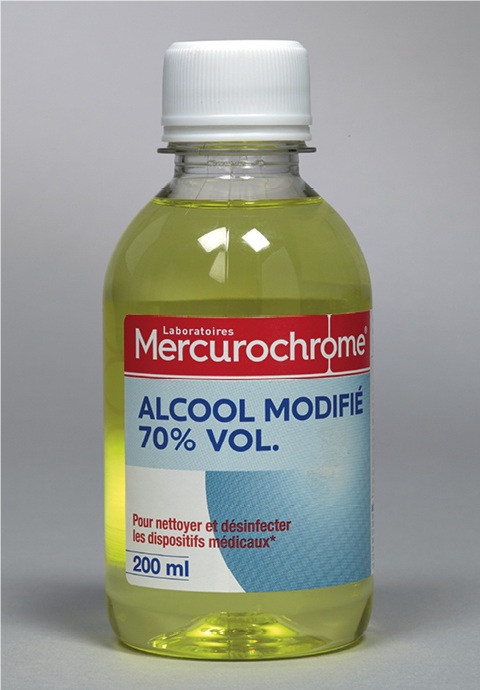
\includegraphics[scale=0.81]{Images/Alcool_pharma.png}
\end{center}
\end{doc}
\begin{doc}{Variation de la masse volumique d’un mélange eau-éthanol en fonction du pourcentage volumique en éthanol}
\vspace{-1cm}
\begin{center}
    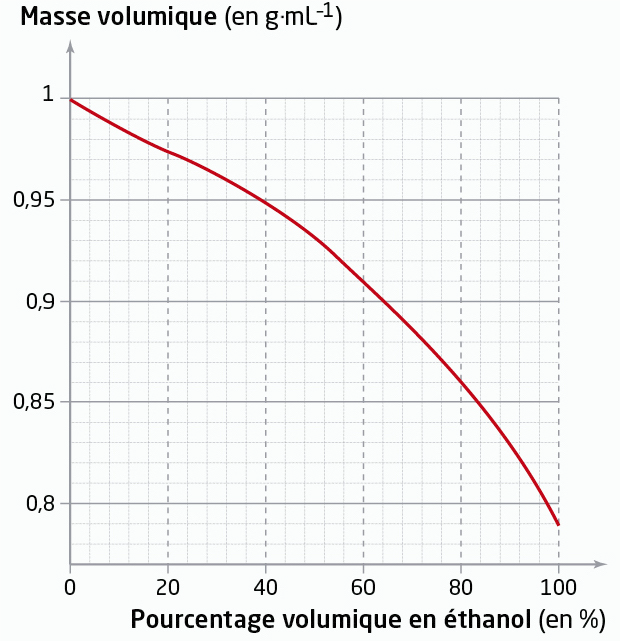
\includegraphics[scale=0.75]{Images/Masse_vol_ethanol.png}
\end{center}
\end{doc}

\end{multicols}

\newpage

\begin{mdframed}[style=autreexo]
\textbf{\bsc{Liste du matériel}}
\begin{itemize}
    \item un flacon contenant de l'alcool pharmaceutique
    \item une balance
    \item une éprouvette graduée de 10mL
    \item une fiole jaugée de 25mL
    \item une pissette en plastique
    \item un bécher de 25mL 
\end{itemize}
\end{mdframed}


\section{Travail à effectuer}

\question{À l’aide du document 2, déterminer la masse volumique de l’éthanol pur, ainsi que la masse volumique de l’eau.}{Par lecture graphique, on lit $\rho_{eau}=1$~g.mL$^{-1}$ lorsque le pourcentage volumique en éthanol est égal à 0\% et $\rho_{ethanol}=0.79$~g.mL$^{-1}$ lorsque le pourcentage volumique en éthanol est égal à 100\%.}{0}

\question{Proposer un protocole permettant de déterminer expérimentalement la masse volumique de l’alcool pharmaceutique vendu par le pharmacien.}{On pèse la verrerie qu'on va utiliser (bécher, fiole jaugée ou éprouvette graduée). On tare la balance (ou on note la masse de la verrerie pour la soustraire par la suite). On verse un volume V d'alcool pharmaceutique dans la verrerie en s'aidant des traits de graduation de la verrerie. On vérifie que le bas du ménisque coïncide bien avec la graduation. On note le volume versé $V$. On pèse ensuite l'ensemble \{verrerie+alcool\} pour en déduire la masse d'alcool versé.}{0}

\question{Appeler le porfesseur pour valider votre protocole expérimental.}{}{0}

\question{Mettre en \oe uvre le protocole précédent et déterminer la masse volumique de l’alcool pharmaceutique vendu par le pharmacien.}{On pèse l'éprouvette graduée à vide, on remplit d'un certain volume d'alcool pharmaceutique $V$ et on pèse l'ensemble. On en déduit la masse volumique $\rho=\frac{m_{verrerie+eau/ethanol}-m_{verrerie}}{V}$
. On laisse ici le choix de la verrerie, le TP suivant permettra d'appréhender la précision des différents types de verrerie. Mais pour une mesure précise, il faut choisir ici une fiole jaugée.}{0}

\question{La législation autorise un écart de $\pm~2\%$.VOL sur la proportion volumique d'éthanol contenue dans ce produit. Déterminer si l’indication portée sur le flacon d’alcool pharmaceutique vendu est conforme.}{La mesure doit être conforme à la valeur indiquée. Si l'écart entre la mesure et la valeur indiquée est supérieur à 2\%, on peut mettre en cause :
\begin{itemize}
    \item le choix de la verrerie dans le protocole : effectivement, si le choix s'est porté sur le bécher, le volume lu est peu précis (5\% sur la valeur lue au moins),
    \item la quantité réelle d'éthanol contenue : l'éthanol étant volatil, une petite quantité a pu s'évaporer du flacon modifiant la masse volumique du mélange.
\end{itemize}}{0}

\question{L’alcool pharmaceutique vendu par le pharmacien a été préparé en utilisant 75 mL d’eau. Calculer le volume d’éthanol qu’il a fallu ajouter pour fabriquer cet alcool.}{On sait que la proportion volumique en éthanol vaut $x_V=\frac{V_{ethanol}}{V_tot}=70$\%. Comme $V_{tot}=V_{ethanol}+V_{eau}$, on en déduit : 
\begin{align*}
    \frac{V_{ethanol}}{V_{ethanol}+V_{eau}} &= 0,70 \\
    V_{ethanol} &= 0,70\times (V_{ethanol}+V_{eau}) \\
    V_{ethanol}\times (1-0,70) &= V_{eau} \\
    V_{ethanol}  &= \frac{V_{eau}}{1-0,70} = \frac{75~\text{mL}}{1-0,70}=250~\text{mL}
\end{align*}}{0}

  %%%%%%%%%% Devoirs Notés %%%%%%%%%%
  %\modeCorrection

\nomPrenomClasse

\begin{center}
\begin{Large}
    
    Interrogation de cours : Corps purs et mélanges au quotidien (10min)
\end{Large}
\end{center}
\vspace{1cm}


\question{Définir un corps pur. Donner un exemple.}{un corps pur est constitué d'une unique espèce chimique. On peut prendre l'exemple de l'eau pure ou du graphite.}{2}

\question{Dans un récipient, on verse de l'huile et de l'eau. Qualifier le mélange obtenu. Comment peut-on qualifier les deux liquides ?}{Le mélange obtenu est hétérogène. Les deux liquides ne sont pas miscibles.}{2}

\question{Donner la formule de la masse volumique. Donner la signification et l'unité de chaque grandeur physique.}{La masse volumique est donnée par la formule :
\begin{equation*}
    \rho = \frac{m}{V}
\end{equation*} avec $\rho$ la masse volumique (en g.cm$^{-3}$ ou g.L$^{-1}$), avec $m$ la masse (en g ou kg) et V le volume de l'espèce chimique (en cm$^3$ ou m$^3$ ou L ou mL).}{3}
\\
\newline
\newline

\setcounter{exercice}{0}
\nomPrenomClasse

\begin{center}
\begin{Large}
    
    Interrogation de cours : Corps purs et mélanges au quotidien (10min)
\end{Large}
\end{center}
\vspace{1cm}


\question{Définir un mélange. Donner un exemple.}{Un mélange est constitué de plusieurs espèces chimiques. On peut prendre l'exemple de l'huile ou du miel.}{2}

\question{Dans un récipient, on verse de l'huile et beaucoup de poivre. Qualifier le mélange obtenu. Comment qualifier deux liquides formant un mélange homogène ?}{Le mélange obtenu est hétérogène. Les deux liquides sont miscibles.}{2}

\question{Donner la formule de la masse volumique. Donner la signification et l'unité de chaque grandeur physique.}{La masse volumique est donnée par la formule :
\begin{equation*}
    \rho = \frac{m}{V}
\end{equation*} avec $\rho$ la masse volumique (en g.cm$^{-3}$ ou g.L$^{-1}$), $m$ la masse (en g ou kg) et V le volume de l'espèce chimique (en cm$^3$ ou m$^3$ ou L ou mL).}{3}

  \modeCorrection

\nomPrenomClasse

\begin{center}
\begin{Large}
    
    Interrogation de cours : Corps purs et mélanges au quotidien (10min)
\end{Large}
\end{center}
\vspace{1cm}


\question{Citer un test chimique pour reconnaitre la présence de dioxyde de carbone \chemform{CO_2}.}{Le \chemform{CO_2} réagit avec l'eaux de chaux pour former un précipité blanc. L'eau de chaux se trouble donc en présence de \chemform{CO_2}.}{2}

\question{L'acétone est miscible avec l'eau. Que cela veut-il dire ? Citer deux espèces chimiques non miscibles.}{Le mélange eau-acétone est homogène. L'huile et l'eau ne sont pas miscibles. On pourrait également citer le graphite avec de l'huile par exemple.}{2}

\question{Donner la formule de la densité d'une espèce chimique. Donner la signification et l'unité de chaque grandeur physique introduite (y compris la densité).}{La densité $d$ d'une espèce chimique est donnée par la formule :
\begin{equation*}
    d = \frac{\rho_{\text{espèce}}}{\rho_{eau}}
\end{equation*} avec $\rho$ la masse volumique (en g.cm$^{-3}$ ou g.L$^{-1}$). La densité s'exprime sans unité.}{3}
\\
\newline
\newline
  %\input{DM/DM1}
  %%\modeCorrection


\renewcommand{\thesubsection}{\textcolor{red}{\Roman{section}.\arabic{subsection}}}
\renewcommand{\thesubsubsection}{\textcolor{red}{\Roman{section}.\arabic{subsection}.\alph{subsubsection}}}
\renewcommand{\titreDocu}[1]{
  \refstepcounter{document} % update counter
  \textbf{Exercice \arabic{document} -- #1} 
  \addcontentsline{toc}{document}{\protect\numberline{} #1} % update table of content
}

\setcounter{section}{0}
\setcounter{document}{0}


\nomPrenomClasse
\vspace{1cm}

\begin{center}
\begin{mdframed}[style=titr, leftmargin=60pt, rightmargin=60pt, innertopmargin=7pt, innerbottommargin=7pt, innerrightmargin=8pt, innerleftmargin=8pt]
\begin{center}
\begin{Large}
    Devoir Surveillé : Corps purs et mélanges au quotidien (55min)
\end{Large}
\end{center}
\end{mdframed}
\end{center}
\vspace{1cm}

\begin{tableauCompetences}
    APP & S'approprier les informations d'un document & & & & \\
    \hline
    REA & Utiliser les pourcentages et les fractions  & & & & \\
     \hline 
    ANA &  Exploiter les informations extraites des données & & & & \\
    \hline
    VAL & Valider/critiquer un modèle & & & &
\end{tableauCompetences}

\begin{tcolorbox}[colback=red!5!white,colframe=red!75!black,title=\textbf{Consignes : }]
   \begin{enumerate}
       \item Vous rendrez l'énoncé avec votre copie de rédaction.
       \item Lisez-bien l'énoncé des exercices. Les questions sont pour la plupart indépendantes. Si vous bloquez sur une question, passez à la suivante,
       \item N'oubliez pas les unités dans vos résultats.
   \end{enumerate}
\end{tcolorbox}

\begin{doc}{Le cyclohexane \begin{large}
    /9,5 points
\end{large}}
Le cyclohexane est une espèce chimique incolore très utilisée en chimie organique pour la synthèse d'arôme artificiel par exemple.
\begin{center}
    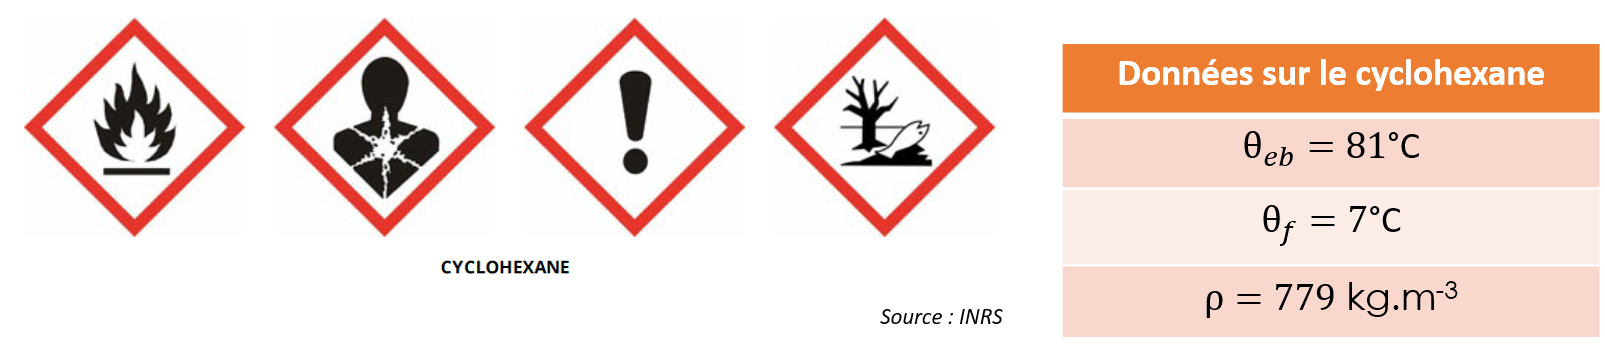
\includegraphics[scale=0.5]{Images/Cyclohexane.png}
\end{center}

\question{Représenter deux pictogrammes de sécurité sur votre copie et donner leur signification. (2pts)}{De gauche à droite sur la figure : inflammable, toxicité aigu (agent CMR), irritant/nocif, pollue l'environnement.}{0}
%\\
\question{Le cyclohexane est très volatil (il s'évapore à l'air libre). Quels sont les Equipements de Protection Individuels (EPI) à utiliser pour manipuler ce produit ? (1pt)}{Blouse, gants, lunettes et hotte protectrice (car volatil).}{0}
%\\
\question{Donner la signification \underline{précise} du symbole \og $\theta_{f}$ \fg. (1pt)}{Il s'agit de la température de fusion, c'est-à-dire la température à partir de laquelle le cyclohexane devient liquide.}{0}
%\\
\question{Avec quel instrument peut-on mesurer $\theta_{f}$ ? (1pt)}{Avec un banc Kofler (attention à l'écriture).}{0}
%\\
\question{Justifier que le cyclohexane est liquide à la température $T=20\degreCelsius$. (1pt)}{D'après les données fournies, la température de 20$\degreCelsius$ est supérieure à la température de fusion $\theta_{f}$ et inférieure à la température d'ébullition $\theta_{eb}$. Le cyclohexane est donc bien liquide.}{0}
%\\
\question{Citer la masse volumique de l'eau en kg.m$^{-3}$.(0,5pt)}{La masse volumique de l'eau est $\rho_{eau}=1000$~kg.m$^{-3}$.}{0}
%\\
\question{En déduire la densité $d$ du cyclohexane. (1pt)}{La densité du cyclohexane est donc :
\begin{equation*}
    d = \frac{779}{1000}=0,779
\end{equation*}}{0}
%\\
\question{Sachant que le cyclohexane \underline{n'est pas miscible} avec l'eau, schématiser une éprouvette graduée avec un mélange eau-cyclohexane (2pts).}{\begin{center}
    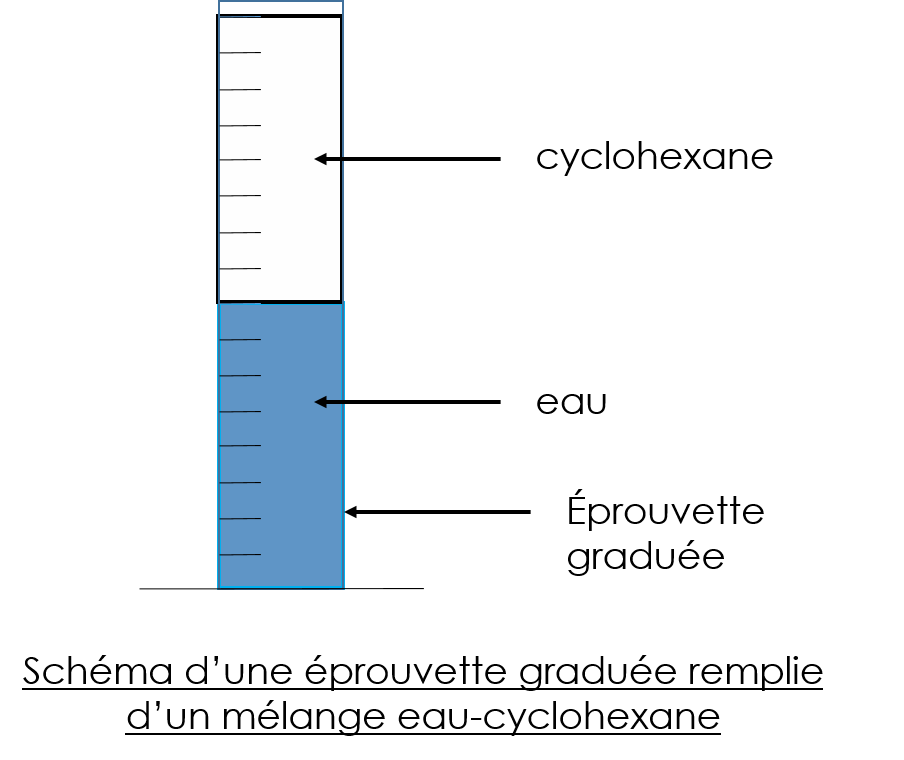
\includegraphics[scale=0.5]{Images/Eprouvette_solution.png}
\end{center}}{0}
\end{doc}

\begin{doc}{L'huile essentielle d'orange\begin{Large}
    /4,5 points
\end{Large}}
\begin{wrapfigure}{r}{0.3\textwidth}
\vspace{-1cm}
    \centering
      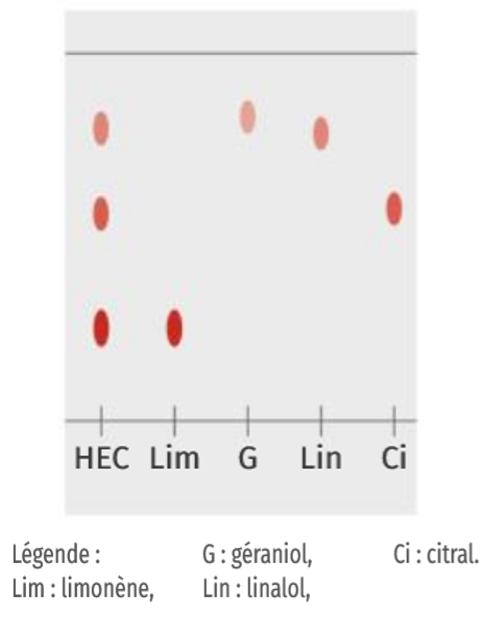
\includegraphics[scale=0.65]{Images/CCm_HEO_3.png}
  \end{wrapfigure}
L'huile essentielle de citron (notée HEC) est obtenue par un procédé mécanique appelé \og extraction par expression à froid\fg~. Cette technique est réservée spécifiquement aux agrumes en raison de la localisation de leurs huiles essentielles (principalement dans la peau).\\
On réalise une CCM afin d'identifier les espèces chimiques présentes dans ces huiles essentielles. Le résultat de la CCM est observable sur la figure de gauche.\\

\question{Rappeler la signification du sigle \og CCM \fg. (0,5pt)}{CCM = Chromatographie sur Couche Mince}{0}
%\\
\question{Que permet de faire la CCM ? (1pt)}{La chromatograpie sur couche mince permet de \textbf{séparer} et d'\textbf{identifier} des espèces chimiques au sein d'un mélange homogène.}{0}
%\\
\question{En vous appuyant sur le résultat de la CCM, justifier que l'huile essentielle de citron (HEC) est un mélange. (1pt)}{On voit apparaître 3 tâches lors de la migration des espèces avec l'éluant correspondant à trois espèces chimiques différentes contenues dans HEC. HEC est donc composé de plusieurs espèces chimiques ce qui est la définition d'un mélange.}{0}
%\\
\question{En vous appuyant sur la légende de la figure, déterminer les espèces chimiques présentes dans l'huile essentielle de citron. (2pts)}{En regardant les espèces avec un même rapport frontal que ceux présents dans HEC, on en déduit qu'il y a du limonène, du linalol et du citral dans HEC.}{0}
\end{doc}

\begin{doc}{Les solutions antisceptiques \begin{Large}
    /6 points
\end{Large}}
Les solutions d’eau oxygénée sont des mélanges d’eau et de peroxyde d’hydrogène \chemform{H_2O_2}. Les solutions d’eau oxygénée à usage domestique, utilisées pour nettoyer et désinfecter les plaies, ont généralement un pourcentage en masse de peroxyde d’hydrogène égal à 3\%. Cependant, les solutions d’eau oxygénée à usage industriel sont plus concentrées : leur pourcentage en masse de peroxyde d’hydrogène peut atteindre 30\%, et même plus.\\

La courbe ci-dessous représente l’évolution de la masse volumique d’une solution d’eau oxygénée en fonction de sa proportion (ou pourcentage) en masse de peroxyde d’hydrogène :

\begin{center}
    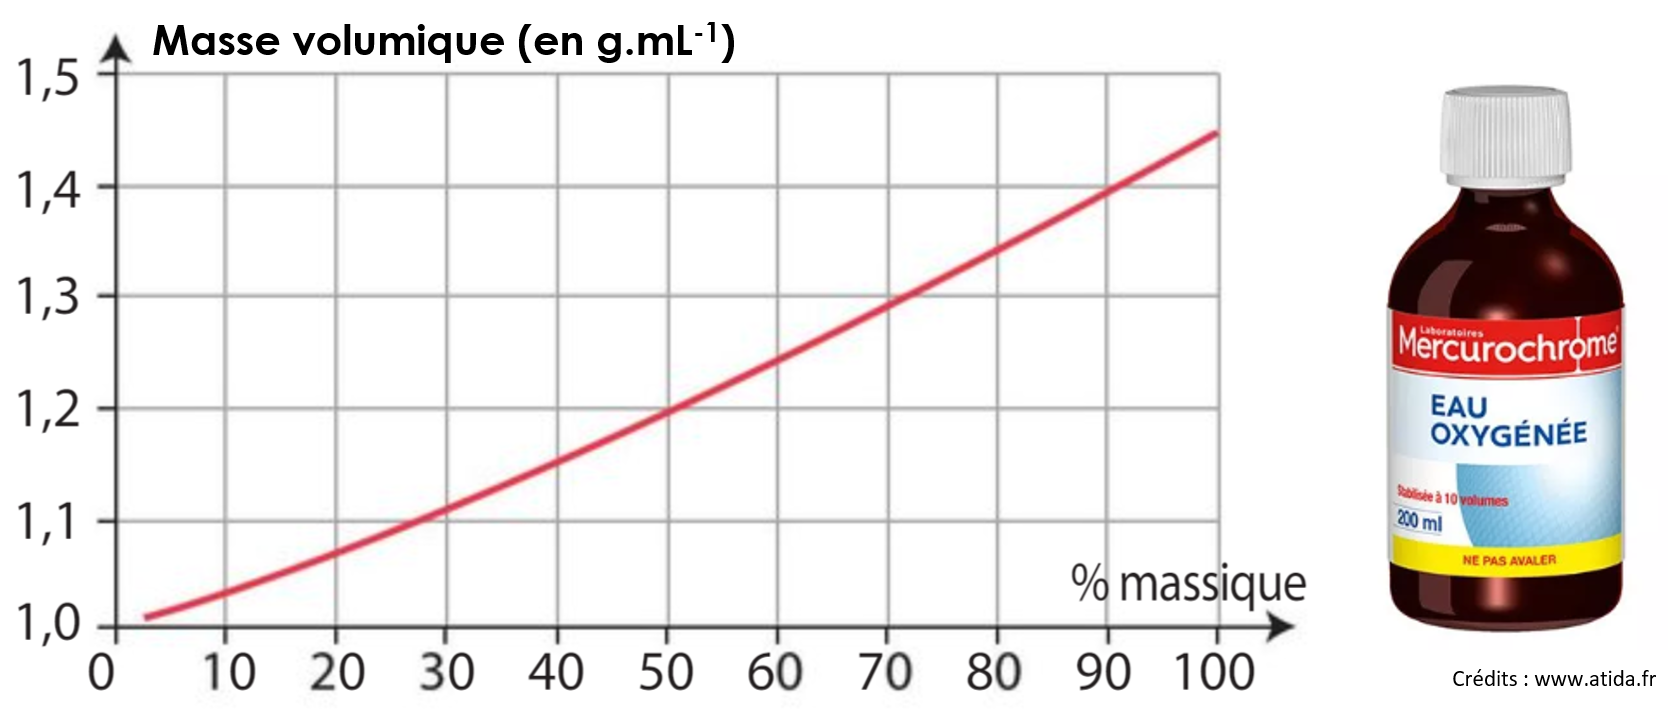
\includegraphics[scale=0.4]{Images/Peroxyde_hydrogene.png}
\end{center}

Afin de déterminer le pourcentage en masse de peroxyde d’hydrogène d’une solution d’eau oxygénée à usage industriel, on détermine la masse d’un volume $V_{H_2O_2} = 25$~mL de cette solution : $m_{H_2O_2} = 30$~g.\\
\question{Nommer le matériel qu'il faut utiliser pour réaliser les mesures précédentes. (2pts)}{Pour mesurer la masse : une balance. Pour mesurer un volume, une éprouvette graduée ou une fiole jaugée (qui est plus précise).}{0}
%\\
\question{Calculer la masse volumique $\rho_{indus}$ de la solution d’eau oxygénée à usage industriel étudiée. (1pt)}{On sait d'après le cours que $\rho=\frac{m}{V}$ soit avec les notations de l'énoncé : $\rho_{indus}=\frac{m_{H_2O_2}}{V_{H_2O_2}}=\frac{30}{25}=1,2$~g.mL$^{-1}$.}{0}
%\\
\question{Déterminer graphiquement la proportion (ou pourcentage) en masse de peroxyde d’hydrogène de la solution d’eau oxygénée à usage industriel étudiée. (1,5pt)}{A l'aide du graphique, on lit un pourcentage en masse pour une masse volumique de $1,2$~g.mL$^{-1}$ égale à 50\%.}{0}
%\\
\question{Calculer le volume de solution d’eau oxygénée à usage industriel contenant $m_2=16$~g de peroxyde d’hydrogène. (1,5pts)}{On sait que la masse volumique correspondante est $\rho_{indus}=1,2$~g.mL$^{-1}$. On en déduit $V=\frac{m_2}{\rho_{indus}}=\frac{16}{1,2}=13$~mL.}{0}
\end{doc}
\newpage
\begin{doc}{La face cachée de l'iceberg  \begin{Large}
    /5 points
\end{Large}}
\begin{wrapfigure}{r}{0.3\textwidth}
\vspace{-1cm}
    \centering
      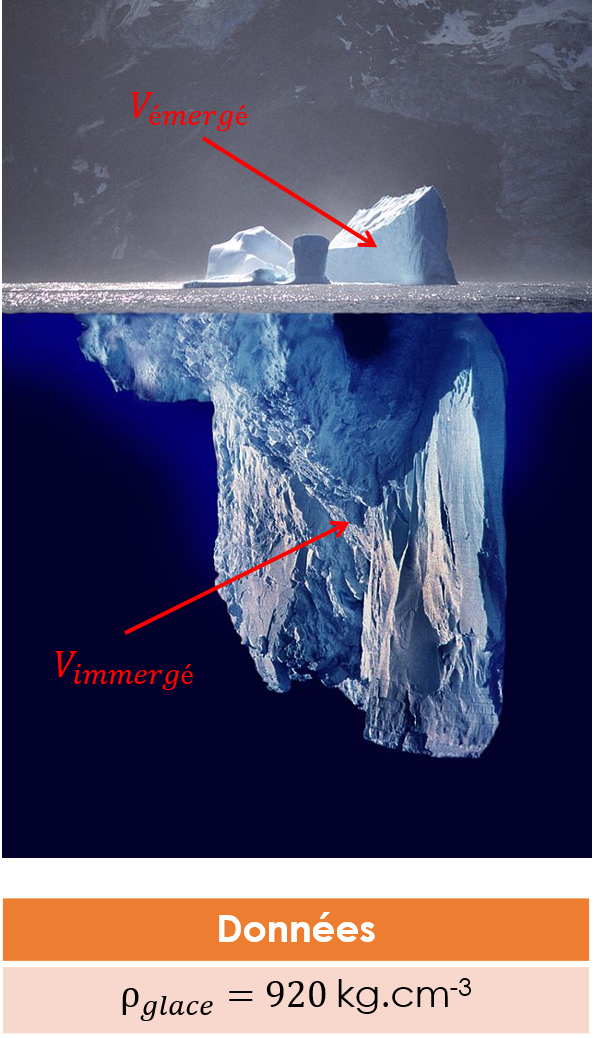
\includegraphics[scale=0.5]{Images/Iceberg.png}
  \end{wrapfigure}
On appelle \og volume immergé \fg, noté $V_{\text{immergé}}$, d'un iceberg le volume de cet iceberg se situant sous l'eau. De même, on appelle \og volume émergé \fg~ d'un iceberg la partie de cette iceberg flottante sur l'eau. Un petit modèle mécanique permet d'établir :
\begin{equation*}
    \rho_{glace}\times V_{Tot} = \rho_{eau}\times V_{\text{immergé}}
\end{equation*}
avec $V_{Tot}$ le volume total de l'iceberg.\\
\question{Donner la relation entre le volume total $V_{Tot}$ de l'iceberg, $V_{\text{immergé}}$ et $V_{\text{émergé}}$. (1pt)}{$V_{Tot}=V_{\text{immergé}}+V_{\text{émergé}}$}{0}%\\
\question{Déterminer l'expression littérale de la proportion du volume immergé de l'iceberg, noté $x_V(\text{immergé})$, en fonction de $\rho_{glace}$ et $\rho_{eau}$. \`{A} l'aide des données, calculer cette proportion. (3pts)}{La proportion volumique du volume immergé est donné par la formule : 
\begin{equation*}
    x_V(\text{immergé}) = \frac{V_{\text{immergé}}}{V_{Tot}}
\end{equation*}
Soit avec l'équation donnée par l'énoncé :
\begin{equation*}
    x_V(\text{immergé}) = \frac{\rho_{glace}}{\rho_{eau}} = \frac{920}{1000} = 92\%
\end{equation*}}{0}%\\
\question{Valider votre résultat en regardant la figure. (1pts)}{Le résultat obtenu est cohérent avec la partie du volume immergé qu'on peut voir sur la figure.}{0}
\end{doc}


\end{document}